\documentclass[12pt,a4paper]{article}
\usepackage[a4paper, margin=0.8in, headheight=14pt]{geometry}
\usepackage{fontspec}
\usepackage{unicode-math}
\setmainfont{TeX Gyre Pagella}
\setmonofont[Scale=0.88]{TeX Gyre Cursor}
\setmathfont{Latin Modern Math}
\usepackage{xcolor}
\usepackage{colortbl}
\usepackage{titlesec}
\usepackage{enumitem}
\usepackage{tabularx}
\usepackage{booktabs}
\usepackage{array}
\usepackage{amsmath}
\allowdisplaybreaks
\usepackage{tikz}
\usetikzlibrary{shapes.geometric, arrows.meta, positioning, calc, fit, decorations.pathreplacing, decorations.pathmorphing, patterns, backgrounds}
% circuitikz not required for this subject
\usepackage{tcolorbox}
\tcbuselibrary{skins, breakable}
\usepackage{etoolbox}
\usepackage{hyperref}
\usepackage{fancyhdr}
\usepackage{graphicx}
\usepackage{microtype}
\hyphenpenalty=10000
\exhyphenpenalty=10000
\sloppy
\usepackage{caption}
\usepackage{setspace}
\usepackage{multirow}
\usepackage{tocloft}
\newcommand{\Q}[1]{\textbf{#1}\par\noindent\ignorespaces}
\definecolor{myred}{RGB}{196,30,58}
\definecolor{mydark}{RGB}{30,30,50}
\definecolor{mygreen}{RGB}{14,120,80}
\definecolor{myteal}{RGB}{0,130,140}
\definecolor{myamber}{RGB}{220,130,20}
\definecolor{mypurple}{RGB}{90,40,140}
\definecolor{mygray}{RGB}{248,249,251}
\definecolor{mgframe}{RGB}{215,220,230}
\definecolor{watermark}{RGB}{145,150,170}
\definecolor{hdrred}{RGB}{250,232,235}
\definecolor{hdrgreen}{RGB}{220,244,233}
\definecolor{hdrteal}{RGB}{220,242,244}
\definecolor{hdramber}{RGB}{253,242,215}
\definecolor{hdrpurple}{RGB}{238,228,255}
\definecolor{hdrgray}{RGB}{238,240,245}
\definecolor{rowalt}{RGB}{250,251,253}
\AfterEndEnvironment{tcolorbox}{\color{mydark}}

\titleformat{\section}{\large\bfseries\color{myred}}{\thesection.}{0.5em}{}[\vspace{1pt}{\color{myred}\rule{\linewidth}{0.8pt}}]
\titleformat{\subsection}{\normalsize\bfseries\color{myteal}}{\thesubsection}{0.5em}{}
\titlespacing*{\section}{0pt}{18pt}{7pt}
\titlespacing*{\subsection}{0pt}{11pt}{4pt}
\setlength{\parindent}{0pt}
\setlength{\parskip}{4pt}
\renewcommand{\cfttoctitlefont}{\large\bfseries\color{myred}}
\renewcommand{\cftaftertoctitle}{\par\noindent{\color{myred}\rule{\linewidth}{0.8pt}}}
\setlength{\cftbeforetoctitleskip}{0pt}
\setlength{\cftaftertoctitleskip}{6pt}
\renewcommand{\cftsecfont}{\normalsize\bfseries\color{mydark}}
\renewcommand{\cftsecpagefont}{\normalsize\bfseries\color{mydark}}
\renewcommand{\cftsecleader}{\cftdotfill{\cftdotsep}}
\setlength{\cftbeforesecskip}{7pt}
\renewcommand{\cftsubsecfont}{\small\color{mydark}}
\renewcommand{\cftsubsecpagefont}{\small\color{mydark}}
\setlength{\cftbeforesubsecskip}{3pt}
\setlength{\cftsubsecindent}{1.4em}
\renewcommand{\cftpartfont}{\normalsize\bfseries\color{myteal}}
\renewcommand{\cftpartpagefont}{\normalsize\bfseries\color{myteal}}
\setlength{\cftbeforepartskip}{14pt}
\renewcommand{\arraystretch}{1.45}
\setlength{\tabcolsep}{6pt}
\arrayrulecolor{mydark}
\newcolumntype{B}[1]{>{\small\bfseries\raggedright\arraybackslash}m{#1}}
\newcolumntype{C}[1]{>{\centering\arraybackslash}m{#1}}
\newcolumntype{Y}{>{\small\raggedright\arraybackslash}X}
\renewcommand{\tabularxcolumn}[1]{m{#1}}
\newcommand{\currmodule}{Module 1}
\pagestyle{fancy}
\fancyhf{}
\fancyhead[L]{\small\color{myred}\textbf{EC303}\;\color{mydark}--- Signals and System}
\fancyhead[R]{\small\color{myteal}\textbf{\currmodule\ Notes}}
\fancyfoot[C]{\small\color{mydark}\thepage}
\fancyfoot[R]{\small\color{watermark}\textit{\copyright\ Biraj}}
\renewcommand{\headrulewidth}{0.5pt}
\renewcommand{\footrulewidth}{0.3pt}

\hypersetup{colorlinks=true, linkcolor=myteal, urlcolor=myteal,
  pdfauthor={Biraj Sarkar},
  pdftitle={EC303 --- Combined Notes}}

\tcbset{
  tikzbox/.style={
    colback=mygray, colframe=mgframe, boxrule=0.6pt, arc=4pt,
    left=8pt, right=8pt, top=6pt, bottom=6pt,
    colbacktitle=mgframe, coltitle=mydark,
    fonttitle=\small\bfseries
  },
  defbox/.style={
    colback=hdrgreen, colframe=mygreen, boxrule=0.8pt, arc=4pt,
    left=9pt, right=9pt, top=6pt, bottom=6pt,
    colbacktitle=mygreen, coltitle=white,
    fonttitle=\small\bfseries
  },
  formulabox/.style={
    colback=hdrteal, colframe=myteal, boxrule=0.8pt, arc=4pt,
    left=9pt, right=9pt, top=6pt, bottom=6pt,
    colbacktitle=myteal, coltitle=white,
    fonttitle=\small\bfseries
  },
  examplebox/.style={
    colback=hdramber, colframe=myamber, boxrule=0.8pt, arc=4pt,
    left=9pt, right=9pt, top=6pt, bottom=6pt,
    colbacktitle=myamber, coltitle=white,
    fonttitle=\small\bfseries
  },
  masonbox/.style={
    colback=hdrpurple, colframe=mypurple, boxrule=0.8pt, arc=4pt,
    left=9pt, right=9pt, top=6pt, bottom=6pt,
    colbacktitle=mypurple, coltitle=white,
    fonttitle=\small\bfseries
  },
  exambox/.style={
    colback=hdrpurple, colframe=mypurple, boxrule=1pt, arc=5pt,
    left=10pt, right=10pt, top=8pt, bottom=8pt,
    colbacktitle=mypurple, coltitle=white,
    fonttitle=\bfseries,
    breakable, title after break={\textbf{Frequently Asked / Viva Questions (contd.)}}
  }
}
\tcbset{breakable}
\tcbset{coltext=mydark}
\tcbset{after={\color{mydark}}}

\tikzset{
  sysblock/.style={rectangle, draw=myteal, fill=hdrteal,
    minimum width=2.4cm, minimum height=1.1cm,
    font=\small\bfseries, rounded corners=3pt, line width=0.8pt, align=center},
  sigarrow/.style={-Stealth, thick, color=mydark},
  sigcircle/.style={circle, draw=myred, fill=hdrred, inner sep=2pt, font=\small\bfseries},
  circnode/.style={draw=myred, fill=hdrred, circle, thick, inner sep=1.5pt, font=\small\bfseries},
  arrowline/.style={-{Latex[length=2.5mm]}, thick, color=mydark},
  dashline/.style={thick, dashed, color=myteal}
}

\newcommand{\modulestart}[2]{%
  \clearpage
  \renewcommand{\currmodule}{Module #1}%
  \renewcommand{\theHsection}{mod#1.\arabic{section}}%
  \renewcommand{\theHsubsection}{\theHsection.\arabic{subsection}}%
  \renewcommand{\theHsubsubsection}{\theHsubsection.\arabic{subsubsection}}%
  \phantomsection
  \addcontentsline{toc}{part}{Module #1: #2}%
  \setcounter{section}{0}%
  \begin{center}
    \vspace*{1.0cm}
    {\Huge\bfseries\color{myred} Module #1}\\[10pt]
    {\Large\bfseries\color{mydark} #2}\\[10pt]
    {\color{myred}\rule{0.55\linewidth}{1.2pt}}
  \end{center}
  \vspace{14pt}
}
\begin{document}

\thispagestyle{empty}

% ─── Page Border (TikZ Overlay) ────────────────────────────────────────────────
\begin{tikzpicture}[remember picture, overlay]
  % Outer border (fine line in mgframe)
  \draw[color=mgframe, line width=1.5pt] 
    ($(current page.north west) + (0.6in, -0.6in)$) rectangle 
    ($(current page.south east) + (-0.6in, 0.6in)$);
  % Inner border (finer accent line in myred)
  \draw[color=myred, line width=0.8pt] 
    ($(current page.north west) + (0.65in, -0.65in)$) rectangle 
    ($(current page.south east) + (-0.65in, 0.65in)$);
\end{tikzpicture}

\vspace*{1.0cm}
\begin{center}
  {\Huge\bfseries\color{myred} EC303}\\[10pt]
  {\LARGE\bfseries\color{mydark} Signals and System}\\[20pt]
  {\color{myred}\rule{0.7\linewidth}{1.5pt}}\\[18pt]
  {\Large\color{myteal}\textbf{Combined Module Notes}}\\[8pt]
  {\large\color{mydark} Modules 1 -- 5}\\[40pt]
  {\normalsize\color{mydark} Semester III \quad$\bullet$\quad ECE \quad$\bullet$\quad 3 Credits}\\[12pt]
  {\normalsize\color{mydark} CGEC \;$|$\; B.Tech ECE (2023--27)}
\end{center}
\vspace{1.0cm}
\begin{center}
  \begin{tcolorbox}[colback=mygray, colframe=mgframe, boxrule=0.5pt, arc=3pt, width=0.85\linewidth]
    \centering\small\color{mydark}
    \textbf{Disclaimer / Study Guide Notice:}\\
    These are condensed \textbf{Short Notes} focusing on core theory, key formulas, block/circuit diagrams, and standard viva Q\&As for university exam revision. Exhaustive numerical practice problems and derivation edge cases are not covered. This serves as a quick-revision reference guide for students.
  \end{tcolorbox}
\end{center}
\vfill
\vspace{0.6cm}
\begin{center}
  {\large\bfseries\color{mypurple} Biraj Sarkar}\\[16pt]
  {\footnotesize\color{watermark}\textbf{IN ASSOCIATION WITH}}\\[8pt]
  {\small\bfseries\color{mydark} MAKAUT Wingman \quad$\bullet$\quad MAKAUT Future Minds}\\[12pt]
  {\large\bfseries\color{myteal} Cooch Behar Government Engineering College}
\end{center}
\vfill
\begin{center}{\small\color{watermark}\textit{Exam-Ready Notes}}\end{center}
\clearpage

\hypersetup{linkcolor=mydark}
\tableofcontents
\hypersetup{linkcolor=myteal}
\clearpage

% -- Module 1 -----------------------------------------------------------------
\modulestart{1}{Signals and Systems in Engineering and Science}

\section{Signals and Systems in Engineering and Science}
% ===============================================================================

\subsection{Basic Definitions}
\begin{tcolorbox}[defbox, title={\textbf{Definition: Signal and System}}]
\begin{itemize}[leftmargin=*, itemsep=4pt]
  \item \textbf{Signal:} A physical quantity that varies with one or more independent variables (such as time $t$, spatial coordinates $x, y, z$, or frequency $\omega$) and conveys information regarding the state or behavior of a physical phenomenon. Mathematically, a signal is represented as a single-valued function of independent variable(s), e.g., voltage $v(t)$, acoustic pressure $p(t)$, or pixel intensity matrix $I(x,y)$.
  \item \textbf{System:} An interconnection of physical components, mathematical operators, or software algorithms that accepts an excitation/input signal $x(t)$ or $x[n]$ and produces a corresponding response/output signal $y(t)$ or $y[n]$ according to a well-defined transformation rule:
  \begin{equation}
    y(t) = \mathcal{T}\{x(t)\} \quad \text{or} \quad y[n] = \mathcal{T}\{x[n]\}
  \end{equation}
\end{itemize}
\end{tcolorbox}

\subsection{Real-World Engineering and Scientific Applications}
\begin{itemize}[leftmargin=*, itemsep=3pt]
  \item \textbf{Biomedical Engineering:} Electrocardiogram (ECG) capturing cardiac electrical dipole potentials; Electroencephalogram (EEG) recording neuro-electrical cortical oscillations; photoplethysmogram (PPG) sensing arterial blood volume changes.
  \item \textbf{Telecommunication Systems:} Radio-frequency (RF) modulated electromagnetic waves transmitting digitized speech, video bitstreams, and satellite downlink carrier signals through multipath fading channels.
  \item \textbf{Control and Automation:} Robotic arm angular position feedback sensed by optical encoders; cruise control velocity tracking loops; chemical process temperature/pressure control systems.
  \item \textbf{Geophysics and Seismology:} Primary ($P$) and secondary ($S$) acoustic shear waves recorded by three-axis seismographs for earthquake hypocenter localization and subterranean hydrocarbon reservoir mapping.
  \item \textbf{Speech and Acoustic Processing:} Continuous-time acoustic pressure variations captured by microphones, filtered through anti-aliasing networks, and converted into discrete speech feature vectors for automated speech recognition.
\end{itemize}

\begin{tcolorbox}[tikzbox, title={\textbf{General Input-Output System Architecture}}]
\begin{center}
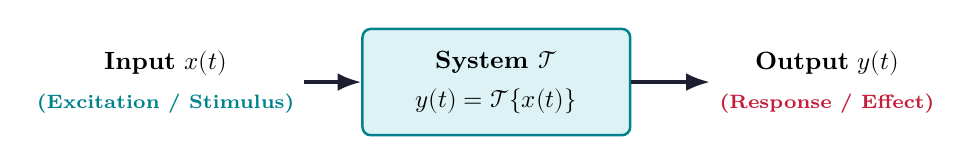
\begin{tikzpicture}[>=Latex, font=\small]
  % Input Node
  \node[align=center] (in) at (-4.2, 0) {
    \textbf{Input} $x(t)$\\[3pt]
    {\scriptsize\color{myteal}\textbf{(Excitation / Stimulus)}}
  };

  % Central System Block
  \node[sysblock, minimum width=3.4cm, minimum height=1.35cm, line width=0.9pt, align=center] (sys) at (0, 0) {
    \textbf{System} $\boldsymbol{\mathcal{T}}$\\[3pt]
    $y(t) = \mathcal{T}\{x(t)\}$
  };

  % Output Node
  \node[align=center] (out) at (4.2, 0) {
    \textbf{Output} $y(t)$\\[3pt]
    {\scriptsize\color{myred}\textbf{(Response / Effect)}}
  };

  % Connecting Arrows with ample clearance
  \draw[->, very thick, color=mydark, -{Latex[length=3mm]}] (in.east) -- (sys.west);
  \draw[->, very thick, color=mydark, -{Latex[length=3mm]}] (sys.east) -- (out.west);
\end{tikzpicture}
\end{center}
\end{tcolorbox}

% ===============================================================================
\section{Classification of Signals}
% ===============================================================================

Signals are classified based on the continuity of their independent variable (time) and dependent variable (amplitude), their periodicity, symmetry, and energy/power distribution.

\subsection{Continuous-Time (CT) vs. Discrete-Time (DT) Signals}
\begin{itemize}[leftmargin=*, itemsep=3pt]
  \item \textbf{Continuous-Time (CT) Signals:} The independent variable $t$ is continuous and defined across an uncountable continuum of real numbers ($t \in \mathbb{R}$). Represented mathematically as $x(t)$.
  \item \textbf{Discrete-Time (DT) Signals:} The independent variable $n$ is defined strictly at discrete integer index points ($n \in \mathbb{Z}$). Often generated by sampling an underlying CT signal at uniform sampling intervals $T_s$, such that $x[n] = x(n T_s)$.
\end{itemize}

\subsection{Continuous-Amplitude vs. Discrete-Amplitude Signals}
\begin{itemize}[leftmargin=*, itemsep=3pt]
  \item \textbf{Continuous-Amplitude Signals (Analog Signals):} The signal amplitude can assume any arbitrary value within a continuous dynamic range $[V_{\min}, V_{\max}]$.
  \item \textbf{Discrete-Amplitude Signals (Quantized / Digital Signals):} The signal amplitude is constrained to a finite, discrete set of predetermined quantization levels $L = 2^b$, where $b$ is the number of encoding bits.
\end{itemize}

\subsection{Periodic vs. Aperiodic Signals}
\begin{tcolorbox}[defbox, title={\textbf{Periodicity Criteria in Continuous and Discrete Time}}]
\begin{itemize}[leftmargin=*, itemsep=4pt]
  \item \textbf{Continuous-Time Periodicity:} A signal $x(t)$ is periodic if there exists a positive non-zero constant $T_0 > 0$ such that:
  \begin{equation}
    x(t + T_0) = x(t) \quad \forall t \in \mathbb{R}
  \end{equation}
  The smallest such positive value $T_0$ is the \textbf{fundamental period} (in seconds), with fundamental angular frequency $\omega_0 = \frac{2\pi}{T_0}$ (rad/s) and cyclic frequency $f_0 = \frac{1}{T_0}$ (Hz).
  \item \textbf{Discrete-Time Periodicity (Critical Difference):} A discrete-time sequence $x[n]$ is periodic if there exists an integer $N > 0$ such that:
  \begin{equation}
    x[n + N] = x[n] \quad \forall n \in \mathbb{Z}
  \end{equation}
  \textbf{Necessary and Sufficient Condition for DT Sinusoid Periodicity:} For $x[n] = \cos(\omega_0 n + \phi)$ or $e^{j\omega_0 n}$ to be periodic, the ratio of its angular frequency to $2\pi$ must be a strictly \textbf{rational number}:
  \begin{equation}
    \frac{\omega_0}{2\pi} = \frac{m}{N} \implies N = m \left(\frac{2\pi}{\omega_0}\right) \in \mathbb{Z}^+
  \end{equation}
  where $m, N$ are coprime integers. If $\omega_0 / 2\pi$ is irrational (e.g., $\omega_0 = 1$ rad), the DT sinusoid is strictly \textbf{aperiodic}.
\end{itemize}
\end{tcolorbox}

\begin{tcolorbox}[examplebox, title={\textbf{Example: Sum of Periodic Signals in CT vs. DT}}]
\textbf{Case 1 (CT):} $x(t) = \cos\left(\frac{\pi}{3}t\right) + \sin\left(\frac{\pi}{4}t\right)$.
Periods: $T_1 = \frac{2\pi}{\pi/3} = 6\text{ s}$, $T_2 = \frac{2\pi}{\pi/4} = 8\text{ s}$.
Ratio: $\frac{T_1}{T_2} = \frac{6}{8} = \frac{3}{4} \in \mathbb{Q}$ (Rational).
Overall fundamental period $T_0 = \text{LCM}(T_1, T_2) = \text{LCM}(6, 8) = 24\text{ s}$. The sum is \textbf{periodic}.

\textbf{Case 2 (DT):} $x[n] = \cos\left(\frac{3\pi}{7}n\right) + \sin\left(\frac{\pi}{5}n\right)$.
$N_1 = \frac{2\pi(7)}{3\pi} = \frac{14}{3} \implies N_1 = 14$ (for $m=3$).
$N_2 = \frac{2\pi(5)}{\pi} = 10$ (for $m=1$).
Overall period $N_0 = \text{LCM}(14, 10) = 70$ samples. The sum is \textbf{periodic}.
\end{tcolorbox}

\subsection{Even (Symmetric) and Odd (Antisymmetric) Signals}
Every arbitrary signal $x(t)$ can be decomposed uniquely into a sum of an even component $x_e(t)$ and an odd component $x_o(t)$:
\begin{equation}
  x(t) = x_e(t) + x_o(t)
\end{equation}
where:
\begin{equation}
  x_e(t) = \frac{x(t) + x(-t)}{2} = x_e(-t), \qquad x_o(t) = \frac{x(t) - x(-t)}{2} = -x_o(-t)
\end{equation}
\begin{itemize}[leftmargin=*, itemsep=3pt]
  \item For any odd continuous-time signal, $x_o(0) = 0$.
  \item Orthogonality: $\int_{-\infty}^{\infty} x_e(t) x_o(t) dt = 0$.
  \item Total energy of signal: $E_x = E_{x_e} + E_{x_o}$.
\end{itemize}

\subsection{Energy and Power Signals}
\begin{tcolorbox}[defbox, title={\textbf{Energy and Power Signal Definitions and Criteria}}]
\textbf{1. Continuous-Time Signals:}
\begin{itemize}[leftmargin=*, itemsep=3pt]
  \item \textbf{Total Energy ($E$):}
  \begin{equation}
    E = \int_{-\infty}^{\infty} |x(t)|^2 dt
  \end{equation}
  \item \textbf{Average Power ($P$):}
  \begin{equation}
    P = \lim_{T \to \infty} \frac{1}{T} \int_{-T/2}^{T/2} |x(t)|^2 dt
  \end{equation}
  For a strictly periodic signal of period $T_0$: $P = \frac{1}{T_0} \int_{0}^{T_0} |x(t)|^2 dt$.
\end{itemize}

\textbf{2. Discrete-Time Signals:}
\begin{itemize}[leftmargin=*, itemsep=3pt]
  \item \textbf{Total Energy ($E$):} $E = \sum_{n=-\infty}^{\infty} |x[n]|^2$.
  \item \textbf{Average Power ($P$):} $P = \lim_{N \to \infty} \frac{1}{2N+1} \sum_{n=-N}^{N} |x[n]|^2$.
\end{itemize}

\textbf{3. Classification Rules:}
\begin{itemize}[leftmargin=*, itemsep=3pt]
  \item \textbf{Energy Signal:} $0 < E < \infty \implies P = 0$. Finite-duration signals, pulses, and exponentially decaying transients are energy signals.
  \item \textbf{Power Signal:} $0 < P < \infty \implies E = \infty$. Periodic waveforms, constant DC levels, and random noise signals are power signals.
  \item \textbf{Neither Energy Nor Power Signal:} Signals whose energy and power are both infinite, e.g., ramps $r(t) = t u(t)$, growing exponentials $x(t) = e^{at} u(t)$ ($a > 0$).
\end{itemize}
\end{tcolorbox}

% ===============================================================================
\section{Standard Elementary Signals and Signal Operations}
% ===============================================================================

\subsection{Standard Elementary Signals}
\begin{itemize}[leftmargin=*, itemsep=4pt]
  \item \textbf{Unit Impulse / Dirac Delta Function $\delta(t)$:}
  \begin{equation}
    \delta(t) = 0 \quad (t \ne 0), \qquad \int_{-\infty}^{\infty} \delta(t) dt = 1
  \end{equation}
  \textbf{Key Properties of $\delta(t)$:}
  \begin{align}
    \text{Sifting Property:} \quad &\int_{-\infty}^{\infty} x(t) \delta(t - t_0) dt = x(t_0) \\
    \text{Product Property:} \quad &x(t) \delta(t - t_0) = x(t_0) \delta(t - t_0) \\
    \text{Time Scaling:} \quad &\delta(a t) = \frac{1}{|a|} \delta(t) \quad (a \ne 0) \\
    \text{Even Function:} \quad &\delta(-t) = \delta(t)
  \end{align}
  \item \textbf{Discrete-Time Unit Impulse / Kronecker Delta $\delta[n]$:}
  \begin{equation}
    \delta[n] = \begin{cases} 1, & n = 0 \\ 0, & n \ne 0 \end{cases}, \qquad \sum_{n=-\infty}^{\infty} x[n] \delta[n - k] = x[k]
  \end{equation}
  \item \textbf{Unit Step Function $u(t)$ and $u[n]$:}
  \begin{equation}
    u(t) = \begin{cases} 1, & t > 0 \\ 0, & t < 0 \end{cases}, \qquad u[n] = \begin{cases} 1, & n \ge 0 \\ 0, & n < 0 \end{cases}
  \end{equation}
  Relationship: $u(t) = \int_{-\infty}^{t} \delta(\tau) d\tau$, and $\delta(t) = \frac{du(t)}{dt}$. In DT: $\delta[n] = u[n] - u[n-1]$.
  \item \textbf{Unit Ramp Function $r(t)$:} $r(t) = t \cdot u(t) = \int_{-\infty}^t u(\tau) d\tau$.
  \item \textbf{Complex Exponential Signal:} $x(t) = e^{s t} = e^{(\sigma + j\omega)t} = e^{\sigma t}(\cos\omega t + j\sin\omega t)$.
  If $\sigma = 0$, $x(t)$ is a pure sinusoidal oscillator; if $\sigma < 0$, it is a damped sinusoid.
\end{itemize}

\subsection{Transformations of the Independent Variable (Time Operations)}
For an arbitrary continuous-time signal $x(t)$, transformations of the form $y(t) = x(at - b)$ are performed using the strict precedence order:
\begin{enumerate}[label=\arabic*., leftmargin=*]
  \item \textbf{Method 1 (Shift then Scale):} First apply time shift by $b$ to obtain $x(t - b)$, then scale time by $a$ to yield $x(at - b)$.
  \item \textbf{Method 2 (Factorized Form):} Express as $x(a(t - b/a))$. First scale time by $a$ to yield $x(at)$, then shift time by $b/a$ to obtain $x(a(t - b/a))$.
\end{enumerate}
\begin{itemize}[leftmargin=*, itemsep=2pt]
  \item If $b > 0$: Delay / Right-shift by $b$. If $b < 0$: Advance / Left-shift by $|b|$.
  \item If $|a| > 1$: Time compression by factor $|a|$. If $0 < |a| < 1$: Time expansion by factor $1/|a|$.
  \item If $a < 0$: Time reversal (reflection about the $y$-axis) accompanied by scaling.
\end{itemize}

% ===============================================================================
\section{Properties and Classifications of Systems}
% ===============================================================================

A system $\mathcal{T}$ maps an input signal $x(t)$ into an output signal $y(t) = \mathcal{T}\{x(t)\}$. Its fundamental mathematical properties determine its operational capability.

\subsection{Linearity: Additivity and Homogeneity}
\begin{tcolorbox}[defbox, title={\textbf{The Linearity Property and Superposition Principle}}]
A system is linear if and only if it satisfies both \textbf{Additivity} and \textbf{Homogeneity} (Scaling), unified into the \textbf{Superposition Principle}:
\begin{equation}
  \mathcal{T}\{a x_1(t) + b x_2(t)\} = a \mathcal{T}\{x_1(t)\} + b \mathcal{T}\{x_2(t)\} = a y_1(t) + b y_2(t)
\end{equation}
for all arbitrary input signals $x_1(t), x_2(t)$ and complex scalars $a, b \in \mathbb{C}$.

\textbf{Essential Test for Linearity:}
\begin{itemize}[leftmargin=*, itemsep=3pt]
  \item \textbf{Zero-Input Zero-Output Condition:} For every linear system, $x(t) \equiv 0 \implies y(t) \equiv 0$. If a system produces a non-zero output for zero input (e.g., $y(t) = 2x(t) + 3$), it is strictly \textbf{non-linear}.
\end{itemize}
\end{tcolorbox}

\subsection{Time-Invariance (Shift-Invariance)}
\begin{tcolorbox}[defbox, title={\textbf{Time-Invariance (Shift-Invariance) Condition}}]
A system is \textbf{Time-Invariant} (or Shift-Invariant in DT) if a time shift in the input signal produces an identical time shift in the output response without changing the functional waveform:
\begin{equation}
  \text{If } \mathcal{T}\{x(t)\} = y(t), \quad \text{then } \mathcal{T}\{x(t - t_0)\} = y(t - t_0) \quad \forall t_0 \in \mathbb{R}
\end{equation}
\textbf{Standard Two-Step Verification Procedure:}
\begin{enumerate}[label=\arabic*., leftmargin=*]
  \item Calculate the response to a shifted input: $y_1(t) = \mathcal{T}\{x(t - t_0)\}$.
  \item Calculate the shifted original output: $y_2(t) = y(t - t_0)$ (replace all occurrences of $t$ with $t - t_0$).
  \item If $y_1(t) \equiv y_2(t)$ for all $t_0$, the system is \textbf{Time-Invariant}; otherwise, it is \textbf{Time-Variant}.
\end{enumerate}
\textit{Indicator of Time-Variance:} Explicit presence of $t$ as a multiplying coefficient (e.g., $y(t) = t \cdot x(t)$) or time-scaling operations ($y(t) = x(2t)$).
\end{tcolorbox}

\subsection{Causality and Memory}
\begin{itemize}[leftmargin=*, itemsep=3pt]
  \item \textbf{Memoryless (Static) System:} The output at any instant $t_0$ depends strictly on the input applied at that exact same instant $t_0$, i.e., $y(t_0) = f(x(t_0))$ (e.g., purely resistive circuit $v(t) = R \cdot i(t)$).
  \item \textbf{Dynamic (System with Memory):} The output at $t_0$ depends on past or future values of the input (e.g., capacitor $v(t) = \frac{1}{C}\int_{-\infty}^t i(\tau)d\tau$, unit delay $y[n] = x[n-1]$).
  \item \textbf{Causality (Non-Anticipative System):} A system is causal if the output at any time $t_0$ depends exclusively on present and/or past inputs ($t \le t_0$), and is completely independent of future inputs ($t > t_0$):
  \begin{equation}
    x_1(t) = x_2(t) \quad \forall t \le t_0 \implies y_1(t) = y_2(t) \quad \forall t \le t_0
  \end{equation}
  All real-time physical systems operating with time as the independent variable are strictly \textbf{causal}. Non-causal systems (e.g., $y(t) = x(t + 2)$) require future preview and are implementable only in offline / post-processing of recorded data.
\end{itemize}

\subsection{BIBO Stability}
\begin{tcolorbox}[defbox, title={\textbf{Bounded-Input Bounded-Output (BIBO) Stability}}]
A system is BIBO stable if every bounded input signal produces a bounded output response:
\begin{equation}
  |x(t)| \le M_x < \infty \quad \forall t \implies |y(t)| \le M_y < \infty \quad \forall t
\end{equation}
where $M_x, M_y$ are finite positive real numbers.
\begin{itemize}[leftmargin=*, itemsep=3pt]
  \item \textbf{Example of Stable System:} $y(t) = \cos(x(t))$ (since $|y(t)| \le 1$ for all real $x(t)$).
  \item \textbf{Example of Unstable System:} Ideal Integrator $y(t) = \int_{-\infty}^t x(\tau) d\tau$. For bounded input $x(t) = u(t)$ ($|u(t)| \le 1$), the output is a ramp $y(t) = t u(t)$, which grows without bound ($y(t) \to \infty$ as $t \to \infty$).
\end{itemize}
\end{tcolorbox}

\subsection{Invertibility and Physical Realizability}
\begin{itemize}[leftmargin=*, itemsep=3pt]
  \item \textbf{Invertibility:} A system $\mathcal{T}$ is invertible if distinct inputs produce distinct outputs (one-to-one mapping). An inverse system $\mathcal{T}^{-1}$ exists such that cascading $\mathcal{T}$ and $\mathcal{T}^{-1}$ yields the identity system:
  \begin{equation}
    w(t) = \mathcal{T}^{-1}\{\mathcal{T}\{x(t)\}\} = x(t)
  \end{equation}
  Non-invertible systems: $y(t) = x^2(t)$ (loss of sign information), $y(t) = 0$ (destroys all input information).
  \item \textbf{Physical Realizability:} A system is physically realizable if it can be constructed using real physical hardware components (RLC networks, operational amplifiers, DSP microchips). Necessary conditions: Causal, stable or stabilizable, and requires finite energy resources.
\end{itemize}

% ===============================================================================
\newpage
% Quick Revision Page (Mandatory Last Section)
% ===============================================================================

\begin{center}
  {\large\bfseries\color{myred} Quick Revision --- Module 1}\\[3pt]
  {\small\color{mydark}\textbf{Core Formulas, One-Line Definitions \& Viva Questions}}
\end{center}
\vspace{2pt}
\noindent{\color{myred}\rule{\linewidth}{1.2pt}}
\vspace{8pt}

\begin{tcolorbox}[formulabox, title={\textbf{Key Formulas and Mathematical Conditions at a Glance}}]
\par\vspace{4pt}\noindent
\begingroup
\setlength{\tabcolsep}{5pt}
\setlength{\extrarowheight}{3pt}
\renewcommand{\arraystretch}{1.35}
\begin{tabularx}{\linewidth}{|B{5.0cm}|Y|}
\hline
\textbf{Property / Operation} & \textbf{Mathematical Definition / Formula} \\
\hline
CT Signal Energy & $E = \int_{-\infty}^{\infty} |x(t)|^2 dt$ \\
\hline
CT Average Power & $P = \lim_{T \to \infty} \frac{1}{T} \int_{-T/2}^{T/2} |x(t)|^2 dt$ \\
\hline
DT Signal Energy \& Power & $E = \sum_{n=-\infty}^{\infty} |x[n]|^2, \quad P = \lim_{N \to \infty} \frac{1}{2N+1} \sum_{n=-N}^N |x[n]|^2$ \\
\hline
Even and Odd Decomposition & $x_e(t) = \frac{x(t) + x(-t)}{2}, \quad x_o(t) = \frac{x(t) - x(-t)}{2}$ \\
\hline
Dirac Delta Sifting Property & $\int_{-\infty}^{\infty} x(t) \delta(t - t_0) dt = x(t_0)$ \\
\hline
Delta Scaling Property & $\delta(at) = \frac{1}{|a|} \delta(t)$ \\
\hline
DT Sinusoid Periodicity & $\frac{\omega_0}{2\pi} = \frac{m}{N} \in \mathbb{Q} \implies N = m\left(\frac{2\pi}{\omega_0}\right)$ \\
\hline
Linear Superposition & $\mathcal{T}\{a x_1 + b x_2\} = a \mathcal{T}\{x_1\} + b \mathcal{T}\{x_2\}$ \\
\hline
Time-Invariance Test & $\mathcal{T}\{x(t - t_0)\} = y(t - t_0) \quad \forall t_0$ \\
\hline
BIBO Stability Condition & $|x(t)| \le M_x < \infty \implies |y(t)| \le M_y < \infty$ \\
\hline
\end{tabularx}
\endgroup
\end{tcolorbox}

\begin{tcolorbox}[defbox, title={\textbf{One-Line Definitions for Rapid Review}}]
\par\vspace{4pt}\noindent
\begingroup
\setlength{\tabcolsep}{5pt}
\setlength{\extrarowheight}{3pt}
\renewcommand{\arraystretch}{1.35}
\begin{tabularx}{\linewidth}{|B{4.5cm}|Y|}
\hline
\textbf{Concept} & \textbf{One-Line Technical Definition} \\
\hline
Signal & A function of one or more independent variables that conveys physical information. \\
\hline
System & An entity that processes an input signal to yield an output signal according to a transformation rule. \\
\hline
Energy Signal & A signal with finite total energy ($0 < E < \infty$) and strictly zero average power ($P=0$). \\
\hline
Power Signal & A signal with finite non-zero average power ($0 < P < \infty$) and infinite total energy ($E=\infty$). \\
\hline
Dirac Delta Function & An idealized distribution having zero value everywhere except at origin, with unit area under integration. \\
\hline
Linear System & A system that simultaneously obeys the principles of additivity and homogeneity. \\
\hline
Time-Invariant System & A system whose input-output characteristics and parameters do not change with time. \\
\hline
Causal System & A system whose output at any instant depends solely on current and past inputs, never on future inputs. \\
\hline
BIBO Stable System & A system that guarantees a bounded output response whenever excited by a bounded input. \\
\hline
Invertible System & A system where distinct inputs produce distinct outputs, enabling exact recovery of the input. \\
\hline
\end{tabularx}
\endgroup
\end{tcolorbox}

\begin{tcolorbox}[exambox, title={\textbf{Frequently Asked / Viva Questions}}]
\begin{enumerate}[topsep=0pt, label=\textbf{Q\arabic*.}, itemsep=5pt]
  \item \Q{Can a signal be simultaneously an energy signal and a power signal?}
  No. Energy and power signals are mutually exclusive. For an energy signal, $0 < E < \infty$, which forces average power $P = \lim_{T \to \infty} E/T = 0$. For a power signal, $0 < P < \infty$, which implies total energy $E = \int |x(t)|^2 dt = \infty$.

  \item \Q{State whether the discrete-time signal $x[n] = \sin(3n)$ is periodic.}
  No. For a discrete-time sinusoid $\sin(\omega_0 n)$ to be periodic, $\omega_0 / 2\pi$ must be a rational number. Here $\omega_0 = 3$, so $\frac{\omega_0}{2\pi} = \frac{3}{2\pi}$, which is irrational. Hence, $x[n] = \sin(3n)$ is strictly aperiodic.

  \item \Q{What is the physical significance of the Dirac delta function $\delta(t)$?}
  It models an instantaneous impulse of infinite amplitude and infinitesimal duration whose total integrated strength (area) equals unity. It serves as the fundamental probing probe to extract the impulse response of LTI systems.

  \item \Q{Evaluate $\int_{-\infty}^{\infty} (t^3 + 4) \delta(t - 2) dt$.}
  Applying the sifting property $\int x(t)\delta(t - t_0)dt = x(t_0)$ with $t_0 = 2$: the value is $2^3 + 4 = 8 + 4 = 12$.

  \item \Q{Why must a linear system always produce zero output for zero input?}
  By the homogeneity property of linear systems, $\mathcal{T}\{a \cdot x(t)\} = a \cdot \mathcal{T}\{x(t)\}$. Setting scalar $a = 0$ gives $\mathcal{T}\{0 \cdot x(t)\} = 0 \cdot y(t) \implies \mathcal{T}\{0\} = 0$.

  \item \Q{Is the system $y(t) = x(2t)$ time-invariant?}
  No. A shift in input gives $y_1(t) = \mathcal{T}\{x(t - t_0)\} = x(2t - t_0)$, whereas shifting the output gives $y(t - t_0) = x(2(t - t_0)) = x(2t - 2t_0)$. Since $y_1(t) \ne y(t - t_0)$, the system is time-variant.

  \item \Q{Is the accumulator system $y[n] = \sum_{k=-\infty}^n x[k]$ stable?}
  No. For bounded input $x[n] = u[n]$ (where $|x[n]| \le 1$), the output is $y[n] = (n+1)u[n]$, which approaches $\infty$ as $n \to \infty$. A bounded input produces an unbounded output, so it is BIBO unstable.

  \item \Q{Distinguish between continuous-time frequency $\omega$ and discrete-time frequency $\Omega$.}
  In CT, frequency $\omega$ (rad/s) spans $(-\infty, \infty)$ and physical oscillations can be arbitrarily fast. In DT, frequency $\Omega$ (rad/sample) is periodic with period $2\pi$, and distinct frequencies exist only within the range $-\pi \le \Omega < \pi$.

  \item \Q{What is the difference between causal and physically realizable systems?}
  A causal system depends only on present and past inputs. A physically realizable system must be causal, stable (or stabilizable), and capable of being constructed using physical components with finite tolerances and energy.

  \item \Q{What is the total energy of an odd signal in terms of its integral over positive time?}
  Since $|x_o(t)|^2$ is strictly an even function, $E = \int_{-\infty}^{\infty} |x_o(t)|^2 dt = 2 \int_0^{\infty} |x_o(t)|^2 dt$.
\end{enumerate}
\end{tcolorbox}

\begin{tcolorbox}[tikzbox, title={\textbf{Summary Matrix: System Properties and Diagnostic Tests}}]
\par\vspace{4pt}\noindent
\begingroup
\setlength{\tabcolsep}{4.5pt}
\setlength{\extrarowheight}{3pt}
\renewcommand{\arraystretch}{1.35}
\begin{tabularx}{\linewidth}{|B{3.2cm}|B{3.5cm}|Y|}
\hline
\textbf{Property} & \textbf{Governing Equation} & \textbf{Quick Inspection Rule} \\
\hline
Linearity & $\mathcal{T}\{a x_1 + b x_2\} = a y_1 + b y_2$ & Non-linear if constants added ($+c$), powers ($x^2$), transcendental functions ($\sin x$), or $y(0) \ne 0$. \\
\hline
Time-Invariance & $\mathcal{T}\{x(t-t_0)\} = y(t-t_0)$ & Time-variant if explicit $t$ multiplies $x$ ($t x(t)$) or time scaling/reflection ($x(-t), x(2t)$). \\
\hline
Causality & $y(t_0) = f(x(t \le t_0))$ & Non-causal if output depends on future time arguments (e.g., $x(t+1), x[n+2]$). \\
\hline
BIBO Stability & $|x| \le M_x \implies |y| \le M_y$ & Unstable if integration/summation without decay creates infinite accumulation for DC/step inputs. \\
\hline
Memory (Static/Dynamic) & $y(t_0) = f(x(t_0))$ & Static if output depends only on input at current instant; dynamic if delays ($x(t-1)$) or derivatives present. \\
\hline
Invertibility & $\mathcal{T}^{-1}\{\mathcal{T}\{x\}\} = x$ & Non-invertible if multiple inputs map to same output (e.g., $x^2(t), \text{sgn}(x(t)), 0$). \\
\hline
\end{tabularx}
\endgroup
\end{tcolorbox}


% -- Module 2 -----------------------------------------------------------------
\modulestart{2}{Linear Shift-Invariant (LSI) Systems Overview}

\section{Linear Shift-Invariant (LSI) Systems Overview}
% ───────────────────────────────────────────────────────────────────────────────

\begin{tcolorbox}[defbox, title={\textbf{Definition: Linear Shift-Invariant (LSI / LTI) System}}]
A system $\mathcal{T}$ is called a \textbf{Linear Shift-Invariant (LSI)} or \textbf{Linear Time-Invariant (LTI)} system if it satisfies both the principle of \textbf{Linearity} (superposition: additivity and homogeneity) and the condition of \textbf{Shift-Invariance} (time-invariance).

Formally, for arbitrary scalar multipliers $a, b \in \mathbb{C}$ and arbitrary inputs $x_1(t), x_2(t)$:
\begin{enumerate}[topsep=2pt, itemsep=2pt]
  \item \textbf{Superposition (Linearity):} $\mathcal{T}\{a x_1(t) + b x_2(t)\} = a \mathcal{T}\{x_1(t)\} + b \mathcal{T}\{x_2(t)\} = a y_1(t) + b y_2(t)$.
  \item \textbf{Shift-Invariance (Time-Invariance):} If $\mathcal{T}\{x(t)\} = y(t)$, then $\mathcal{T}\{x(t - t_0)\} = y(t - t_0)$ for any arbitrary shift $t_0 \in \mathbb{R}$ (or $n_0 \in \mathbb{Z}$ in discrete-time).
\end{enumerate}
\end{tcolorbox}

\subsection{Representation of Signals Through Shifted Impulses}
Any continuous-time signal $x(t)$ can be viewed as a continuum of weighted, shifted Dirac delta impulses via the sifting property:
\begin{equation}
  x(t) = \int_{-\infty}^{\infty} x(\tau) \delta(t - \tau) d\tau
\end{equation}
Similarly, any discrete-time signal $x[n]$ is exactly decomposed into a linear combination of weighted, shifted Kronecker deltas:
\begin{equation}
  x[n] = \sum_{k=-\infty}^{\infty} x[k] \delta[n - k]
\end{equation}
This decomposition forms the conceptual bedrock of LTI system analysis: because the system is linear and time-invariant, knowledge of its response to a single unit impulse ($\delta(t)$ or $\delta[n]$) is sufficient to completely determine its response to \textit{any arbitrary} input signal.

% ───────────────────────────────────────────────────────────────────────────────
\section{Impulse Response and Step Response}
% ───────────────────────────────────────────────────────────────────────────────

\subsection{The Impulse Response $h(t)$ and $h[n]$}

\begin{tcolorbox}[defbox, title={\textbf{Definition: Impulse Response}}]
The \textbf{Impulse Response} $h(t)$ (in CT) or $h[n]$ (in DT) is the output of an LSI system when the input is a unit impulse applied at the origin under initial rest conditions (zero energy stored in the system):
\begin{align}
  h(t) &\triangleq \mathcal{T}\{\delta(t)\} \quad \text{(Continuous-Time)} \\
  h[n] &\triangleq \mathcal{T}\{\delta[n]\} \quad \text{(Discrete-Time)}
\end{align}
\end{tcolorbox}

\textbf{Physical Significance:}
\begin{itemize}[topsep=2pt, itemsep=2pt]
  \item It acts as the ``fingerprint'' or signature of an LSI system. Every structural attribute—memory, causality, stability, invertibility, and frequency selectivity—is entirely encoded in $h(t)$ or $h[n]$.
  \item It characterizes the transient relaxation dynamics of the physical system following an instantaneous excitation.
\end{itemize}

\subsection{The Step Response $s(t)$ and $s[n]$}

\begin{tcolorbox}[defbox, title={\textbf{Definition: Step Response}}]
The \textbf{Step Response} $s(t)$ (in CT) or $s[n]$ (in DT) is the system output when excited by a unit step function $u(t)$ or $u[n]$ under zero initial state:
\begin{equation}
  s(t) \triangleq \mathcal{T}\{u(t)\}, \qquad s[n] \triangleq \mathcal{T}\{u[n]\}
\end{equation}
\end{tcolorbox}

\subsection{Relationship Between Impulse Response and Step Response}
Since the unit step is the integral (running sum) of the unit impulse:
\begin{equation}
  u(t) = \int_{-\infty}^t \delta(\tau) d\tau, \qquad u[n] = \sum_{k=-\infty}^n \delta[k]
\end{equation}
By linearity and time-invariance, the step response is the running integral (or running sum) of the impulse response:

\begin{tcolorbox}[formulabox, title={\textbf{Fundamental Inter-relationships: Impulse $\leftrightarrow$ Step Response}}]
\textbf{Continuous-Time (CT):}
\begin{equation}
  s(t) = \int_{-\infty}^{t} h(\tau) d\tau \iff h(t) = \frac{ds(t)}{dt}
\end{equation}
\textbf{Discrete-Time (DT):}
\begin{equation}
  s[n] = \sum_{k=-\infty}^{n} h[k] \iff h[n] = s[n] - s[n-1] = \nabla s[n]
\end{equation}
where $\nabla$ denotes the backward difference operator.
\end{tcolorbox}

\begin{tcolorbox}[examplebox, title={\textbf{Derivation Example: Step Response of First-Order RC Circuit}}]
Consider a simple low-pass RC series circuit where input $x(t) = v_{in}(t)$ and output $y(t) = v_C(t)$. The differential equation is $RC \frac{dy(t)}{dt} + y(t) = x(t)$.
\begin{enumerate}[topsep=2pt, itemsep=2pt]
  \item The impulse response is obtained by setting $x(t) = \delta(t)$:
  \begin{equation*}
    h(t) = \frac{1}{RC} e^{-t/RC} u(t)
  \end{equation*}
  \item The step response $s(t)$ is calculated via running integration for $t \ge 0$:
  \begin{equation*}
    s(t) = \int_0^t \frac{1}{RC} e^{-\tau/RC} d\tau = \left[ -e^{-\tau/RC} \right]_0^t = \left( 1 - e^{-t/RC} \right) u(t)
  \end{equation*}
  \item Differentiating $s(t)$ recovers $h(t)$:
  \begin{equation*}
    \frac{ds(t)}{dt} = \frac{1}{RC} e^{-t/RC} u(t) + (1 - e^{-t/RC}) \delta(t) = \frac{1}{RC} e^{-t/RC} u(t) + 0 = h(t) \quad \text{(since } 1-e^0 = 0\text{)}.
  \end{equation*}
\end{enumerate}
\end{tcolorbox}

% ───────────────────────────────────────────────────────────────────────────────
\section{The Convolution Operation}
% ───────────────────────────────────────────────────────────────────────────────

\subsection{Derivation of the Convolution Integral (CT)}
Let a continuous-time LSI system $\mathcal{T}$ have impulse response $h(t) = \mathcal{T}\{\delta(t)\}$.
\begin{enumerate}[topsep=2pt, itemsep=2pt]
  \item Express the input $x(t)$ using the sifting property:
  \begin{equation}
    x(t) = \int_{-\infty}^{\infty} x(\tau) \delta(t - \tau) d\tau
  \end{equation}
  \item Apply the transformation $\mathcal{T}$ to both sides:
  \begin{equation}
    y(t) = \mathcal{T}\{x(t)\} = \mathcal{T}\left\{ \int_{-\infty}^{\infty} x(\tau) \delta(t - \tau) d\tau \right\}
  \end{equation}
  \item By linearity (additivity over continuum and homogeneity for scalar $x(\tau)$):
  \begin{equation}
    y(t) = \int_{-\infty}^{\infty} x(\tau) \mathcal{T}\{\delta(t - \tau)\} d\tau
  \end{equation}
  \item By shift-invariance, $\mathcal{T}\{\delta(t - \tau)\} = h(t - \tau)$:
  \begin{equation}
    y(t) = \int_{-\infty}^{\infty} x(\tau) h(t - \tau) d\tau \triangleq x(t) * h(t)
  \end{equation}
\end{enumerate}

\subsection{Derivation of the Convolution Sum (DT)}
Similarly, for a discrete-time LSI system where $h[n] = \mathcal{T}\{\delta[n]\}$:
\begin{align}
  x[n] &= \sum_{k=-\infty}^{\infty} x[k] \delta[n - k] \\
  y[n] &= \mathcal{T}\{x[n]\} = \sum_{k=-\infty}^{\infty} x[k] \mathcal{T}\{\delta[n - k]\} = \sum_{k=-\infty}^{\infty} x[k] h[n - k] \triangleq x[n] * h[n]
\end{align}

\begin{tcolorbox}[formulabox, title={\textbf{Core Formulation: Convolution Integral and Sum}}]
\begin{align}
  y(t) &= x(t) * h(t) = \int_{-\infty}^{\infty} x(\tau) h(t - \tau) d\tau = \int_{-\infty}^{\infty} h(\tau) x(t - \tau) d\tau \\
  y[n] &= x[n] * h[n] = \sum_{k=-\infty}^{\infty} x[k] h[n - k] = \sum_{k=-\infty}^{\infty} h[k] x[n - k]
\end{align}
\end{tcolorbox}

\subsection{Graphical Interpretation of Convolution}
Evaluating convolution graphically consists of four rigorous sequential steps:
\begin{enumerate}[topsep=2pt, itemsep=3pt]
  \item \textbf{Change of Variable:} Plot $x(\tau)$ and $h(\tau)$ as functions of the dummy variable $\tau$.
  \item \textbf{Folding (Time Reversal):} Flip $h(\tau)$ about the vertical axis to obtain $h(-\tau)$.
  \item \textbf{Shifting (Time Delay):} Shift $h(-\tau)$ by time $t$ to obtain $h(t - \tau)$ (right-shift for $t > 0$, left-shift for $t < 0$).
  \item \textbf{Multiplication and Integration/Summation:} Multiply $x(\tau)$ and $h(t - \tau)$ pointwise, and evaluate the area under the product curve over the overlapping support interval.
\end{enumerate}

\begin{tcolorbox}[tikzbox, title={\textbf{TikZ Illustration: Graphical Convolution Mechanism}}]
\begin{center}
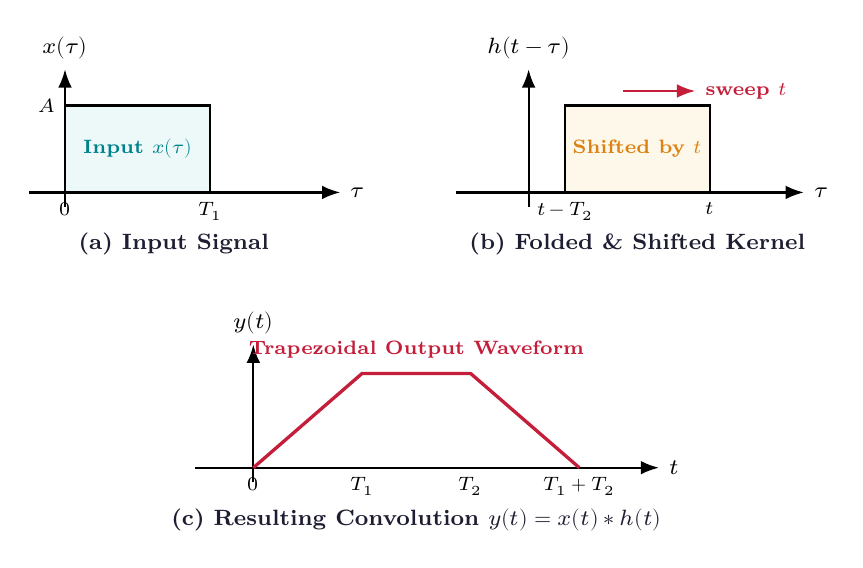
\begin{tikzpicture}[>=Latex, scale=0.92]
  % Step 1: Input x(tau)
  \draw[->, thick] (-0.5,0) -- (3.8,0) node[right] {\footnotesize $\tau$};
  \draw[->, thick] (0,-0.2) -- (0,1.7) node[above] {\footnotesize $x(\tau)$};
  \draw[thick, fill=hdrteal, fill opacity=0.5] (0,0) -- (0,1.2) -- (2,1.2) -- (2,0) -- cycle;
  \node[font=\scriptsize\bfseries, color=myteal] at (1,0.6) {Input $x(\tau)$};
  \node[below] at (0,0) {\scriptsize $0$};
  \node[below] at (2,0) {\scriptsize $T_1$};
  \node[left] at (0,1.2) {\scriptsize $A$};
  \node[below=6pt, font=\footnotesize\bfseries, color=mydark] at (1.5,-0.2) {(a) Input Signal};

  % Step 2: Folded and Shifted h(t - tau)
  \begin{scope}[xshift=6.4cm]
    \draw[->, thick] (-1,0) -- (3.8,0) node[right] {\footnotesize $\tau$};
    \draw[->, thick] (0,-0.2) -- (0,1.7) node[above] {\footnotesize $h(t-\tau)$};
    \draw[thick, fill=hdramber, fill opacity=0.5] (0.5,0) -- (0.5,1.2) -- (2.5,1.2) -- (2.5,0) -- cycle;
    \node[font=\scriptsize\bfseries, color=myamber] at (1.5,0.6) {Shifted by $t$};
    \node[below] at (0.5,0) {\scriptsize $t - T_2$};
    \node[below] at (2.5,0) {\scriptsize $t$};
    \draw[->, myred, thick] (1.3,1.4) -- (2.3,1.4) node[right, myred, font=\scriptsize\bfseries] {sweep $t$};
    \node[below=6pt, font=\footnotesize\bfseries, color=mydark] at (1.5,-0.2) {(b) Folded \& Shifted Kernel};
  \end{scope}

  % Step 3: Overlap & Output
  \begin{scope}[yshift=-3.8cm, xshift=2.6cm]
    \draw[->, thick] (-0.8,0) -- (5.6,0) node[right] {\footnotesize $t$};
    \draw[->, thick] (0,-0.2) -- (0,1.7) node[above] {\footnotesize $y(t)$};
    \draw[very thick, myred] (0,0) -- (1.5,1.3) -- (3.0,1.3) -- (4.5,0);
    \node[below] at (0,0) {\scriptsize $0$};
    \node[below] at (1.5,0) {\scriptsize $T_1$};
    \node[below] at (3.0,0) {\scriptsize $T_2$};
    \node[below] at (4.5,0) {\scriptsize $T_1+T_2$};
    \node[above=2pt, myred, font=\scriptsize\bfseries] at (2.25,1.3) {Trapezoidal Output Waveform};
    \node[below=6pt, font=\footnotesize\bfseries, color=mydark] at (2.25,-0.2) {(c) Resulting Convolution $y(t) = x(t)*h(t)$};
  \end{scope}
\end{tikzpicture}
\end{center}
\end{tcolorbox}

\subsection{Properties of Convolution}

\par\vspace{6pt}\noindent
\begingroup
\setlength{\tabcolsep}{5pt}
\setlength{\extrarowheight}{3pt}
\renewcommand{\arraystretch}{1.4}
\begin{tabularx}{\linewidth}{|B{3.8cm}|Y|Y|}
\hline
\textbf{Property} & \textbf{Continuous-Time Formulation} & \textbf{Discrete-Time Formulation} \\
\hline
Commutative & $x(t) * h(t) = h(t) * x(t)$ & $x[n] * h[n] = h[n] * x[n]$ \\
\hline
Associative & $[x(t) * h_1(t)] * h_2(t) = x(t) * [h_1(t) * h_2(t)]$ & $[x[n] * h_1[n]] * h_2[n] = x[n] * [h_1[n] * h_2[n]]$ \\
\hline
Distributive & $x(t) * [h_1(t) + h_2(t)] = x * h_1 + x * h_2$ & $x[n] * [h_1[n] + h_2[n]] = x * h_1 + x * h_2$ \\
\hline
Shift Property & $x(t - t_1) * h(t - t_2) = y(t - t_1 - t_2)$ & $x[n - n_1] * h[n - n_2] = y[n - n_1 - n_2]$ \\
\hline
Identity Element & $x(t) * \delta(t) = x(t)$ & $x[n] * \delta[n] = x[n]$ \\
\hline
Derivative Property & $\frac{d}{dt}[x(t) * h(t)] = \frac{dx(t)}{dt} * h(t) = x(t) * \frac{dh(t)}{dt}$ & $\nabla[x[n] * h[n]] = \nabla x[n] * h[n] = x[n] * \nabla h[n]$ \\
\hline
Duration Property & If lengths are $L_1$ and $L_2$, duration of $y(t)$ is $L_1 + L_2$. & Number of non-zero samples is $N_1 + N_2 - 1$. \\
\hline
\end{tabularx}
\endgroup

\subsection{Interconnection of LSI Systems}
\begin{itemize}[topsep=2pt, itemsep=3pt]
  \item \textbf{Cascade (Series) Connection:} Equivalent impulse response is the convolution of individual impulse responses:
  \begin{equation}
    h_{eq}(t) = h_1(t) * h_2(t) = h_2(t) * h_1(t)
  \end{equation}
  By the commutative property, the order of cascaded LSI subsystems can be interchanged without altering the overall response.
  \item \textbf{Parallel Connection:} Equivalent impulse response is the arithmetic sum of individual responses:
  \begin{equation}
    h_{eq}(t) = h_1(t) + h_2(t)
  \end{equation}
\end{itemize}

\begin{tcolorbox}[tikzbox, title={\textbf{TikZ Block Diagrams: Cascade and Parallel LSI Interconnections}}]
\begin{center}
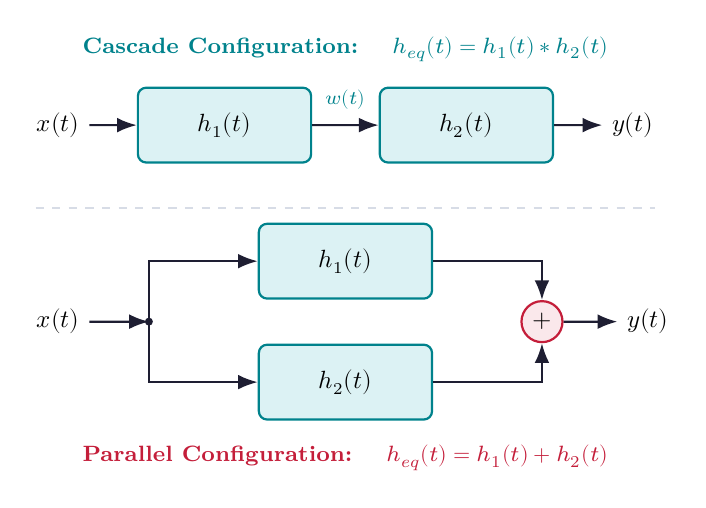
\begin{tikzpicture}[>=Latex, font=\small, scale=0.96]
  % ─── Cascade Configuration ───
  \node[font=\footnotesize\bfseries, color=myteal] at (3.6, 3.0) {Cascade Configuration: \quad $h_{eq}(t) = h_1(t) * h_2(t)$};
  \node (in1) at (-0.2, 2.0) {$x(t)$};
  \node[sysblock, minimum width=2.2cm, minimum height=0.95cm] (sys1) at (2.0, 2.0) {$h_1(t)$};
  \node[sysblock, minimum width=2.2cm, minimum height=0.95cm] (sys2) at (5.2, 2.0) {$h_2(t)$};
  \node (out1) at (7.4, 2.0) {$y(t)$};

  \draw[arrowline] (in1) -- (sys1);
  \draw[arrowline] (sys1) -- node[above=2pt, font=\scriptsize, color=myteal] {$w(t)$} (sys2);
  \draw[arrowline] (sys2) -- (out1);

  % Separator Rule
  \draw[mgframe, dashed, thick] (-0.5, 0.9) -- (7.7, 0.9);

  % ─── Parallel Configuration ───
  \node (in2) at (-0.2, -0.6) {$x(t)$};
  \coordinate (branch) at (1.0, -0.6);
  \node[sysblock, minimum width=2.2cm, minimum height=0.95cm] (p1) at (3.6, 0.2) {$h_1(t)$};
  \node[sysblock, minimum width=2.2cm, minimum height=0.95cm] (p2) at (3.6, -1.4) {$h_2(t)$};
  \node[circnode, inner sep=2pt] (sum) at (6.2, -0.6) {$+$};
  \node (out2) at (7.6, -0.6) {$y(t)$};

  \draw[arrowline] (in2) -- (branch);
  \fill[mydark] (branch) circle (1.5pt);
  \draw[arrowline] (branch) |- (p1.west);
  \draw[arrowline] (branch) |- (p2.west);
  \draw[arrowline] (p1.east) -| (sum.north);
  \draw[arrowline] (p2.east) -| (sum.south);
  \draw[arrowline] (sum) -- (out2);
  \node[font=\footnotesize\bfseries, color=myred] at (3.6, -2.4) {Parallel Configuration: \quad $h_{eq}(t) = h_1(t) + h_2(t)$};
\end{tikzpicture}
\end{center}
\end{tcolorbox}

% ───────────────────────────────────────────────────────────────────────────────
\section{Causality and Stability of LSI Systems}
% ───────────────────────────────────────────────────────────────────────────────

\subsection{Characterization of Causality}
A system is causal if the output at any instant $t_0$ depends only on the input values for $t \le t_0$.

\begin{tcolorbox}[defbox, title={\textbf{Causality Criterion for LSI Systems}}]
A continuous-time (or discrete-time) LSI system is \textbf{causal} if and only if its impulse response is zero for all negative time:
\begin{align}
  \text{CT:} \quad &h(t) = 0 \quad \forall t < 0 \\
  \text{DT:} \quad &h[n] = 0 \quad \forall n < 0
\end{align}
\end{tcolorbox}

\textbf{Proof of Causality Condition:}
The convolution integral gives:
\begin{equation}
  y(t) = \int_{-\infty}^{\infty} h(\tau) x(t - \tau) d\tau = \int_{-\infty}^0 h(\tau) x(t - \tau) d\tau + \int_0^{\infty} h(\tau) x(t - \tau) d\tau
\end{equation}
For $\tau < 0$, the term $t - \tau > t$, representing future input values. Thus, for $y(t)$ to be completely independent of future inputs $x(t - \tau)$ ($\tau < 0$), we must have:
\begin{equation}
  h(\tau) = 0 \quad \text{for all } \tau < 0
\end{equation}
Under causality, the convolution limits simplify to:
\begin{equation}
  y(t) = \int_0^{\infty} h(\tau) x(t - \tau) d\tau = \int_{-\infty}^{t} x(\tau) h(t - \tau) d\tau
\end{equation}
If the input $x(t)$ is also causal ($x(t) = 0$ for $t < 0$):
\begin{equation}
  y(t) = \int_0^t x(\tau) h(t - \tau) d\tau \quad (t \ge 0)
\end{equation}

\subsection{Characterization of BIBO Stability}
A system is Bounded-Input Bounded-Output (BIBO) stable if every bounded input $|x(t)| \le M_x < \infty$ produces a bounded output $|y(t)| \le M_y < \infty$.

\begin{tcolorbox}[formulabox, title={\textbf{BIBO Stability Criterion for LSI Systems}}]
An LSI system is \textbf{BIBO stable} if and only if its impulse response is \textbf{absolutely integrable} (in CT) or \textbf{absolutely summable} (in DT):
\begin{align}
  \text{CT:} \quad &\int_{-\infty}^{\infty} |h(t)| dt < \infty \\
  \text{DT:} \quad &\sum_{n=-\infty}^{\infty} |h[n]| < \infty
\end{align}
\end{tcolorbox}

\begin{tcolorbox}[examplebox, title={\textbf{Rigorous Proof of BIBO Stability Criterion (Sufficiency and Necessity)}}]
\textbf{1. Sufficiency Proof (If $\int |h(t)|dt < \infty \implies$ BIBO Stable):}
Let $|x(t)| \le M_x < \infty$. Taking the magnitude of the output:
\begin{align*}
  |y(t)| &= \left| \int_{-\infty}^{\infty} h(\tau) x(t - \tau) d\tau \right| \le \int_{-\infty}^{\infty} |h(\tau)| \cdot |x(t - \tau)| d\tau \\
  &\le M_x \int_{-\infty}^{\infty} |h(\tau)| d\tau
\end{align*}
Since $\int_{-\infty}^\infty |h(\tau)| d\tau = K < \infty$, we have $|y(t)| \le M_x K < \infty$ for all $t$. Hence, the output is guaranteed bounded.

\textbf{2. Necessity Proof (If BIBO Stable $\implies \int |h(t)|dt < \infty$):}
Suppose $\int_{-\infty}^\infty |h(t)|dt = \infty$. Choose the bounded input:
\begin{equation*}
  x(t - \tau) = \text{sgn}[h(\tau)] = \begin{cases} +1, & h(\tau) > 0 \\ -1, & h(\tau) < 0 \end{cases}
\end{equation*}
Clearly $|x(t)| = 1 \le 1$ is bounded. Then at time $t = 0$:
\begin{equation*}
  y(0) = \int_{-\infty}^{\infty} h(\tau) x(-\tau) d\tau = \int_{-\infty}^{\infty} h(\tau) \text{sgn}[h(\tau)] d\tau = \int_{-\infty}^{\infty} |h(\tau)| d\tau = \infty
\end{equation*}
The output grows unbounded at $t=0$, violating BIBO stability. Therefore, absolute integrability is both necessary and sufficient.
\end{tcolorbox}

% ───────────────────────────────────────────────────────────────────────────────
\section{System Representation Through Differential Equations}
% ───────────────────────────────────────────────────────────────────────────────

\subsection{Linear Constant-Coefficient Differential Equations (LCCDE)}
A continuous-time lumped parameter LTI system is generally modeled by an $N$-th order LCCDE relating input $x(t)$ to output $y(t)$:
\begin{equation}
  \sum_{k=0}^{N} a_k \frac{d^k y(t)}{dt^k} = \sum_{m=0}^{M} b_m \frac{d^m x(t)}{dt^m}
\end{equation}
where $a_k, b_m$ are real, time-invariant coefficients, and $N \ge M$ for physical realizability.

\subsection{Complete Solution: Natural and Forced Responses}
The total output consists of two components:
\begin{equation}
  y(t) = y_h(t) + y_p(t) = y_{zi}(t) + y_{zs}(t)
\end{equation}
\begin{itemize}[topsep=2pt, itemsep=2pt]
  \item \textbf{Homogeneous Solution $y_h(t)$ (Natural Response):} Solution when input $x(t) \equiv 0$:
  \begin{equation}
    \sum_{k=0}^N a_k \frac{d^k y(t)}{dt^k} = 0 \implies \sum_{k=0}^N a_k \lambda^k = 0 \quad \text{(Characteristic Equation)}
  \end{equation}
  If roots $\lambda_i$ are distinct: $y_h(t) = \sum_{i=1}^N C_i e^{\lambda_i t}$.
  \item \textbf{Particular Solution $y_p(t)$ (Forced Response):} The specific response satisfying the non-zero input excitation $x(t)$.
  \item \textbf{Zero-Input Response (ZIR) $y_{zi}(t)$:} Response produced purely by internal stored energy (initial conditions) with zero external input.
  \item \textbf{Zero-State Response (ZSR) $y_{zs}(t)$:} Response produced purely by the input with all initial conditions set to zero: $y_{zs}(t) = x(t) * h(t)$.
\end{itemize}

\subsection{Condition of Initial Rest}
\begin{tcolorbox}[defbox, title={\textbf{Concept: Initial Rest}}]
An LCCDE system is said to be at \textbf{Initial Rest} if the system starts with zero energy storage prior to input application:
\begin{equation}
  \text{If } x(t) = 0 \text{ for } t \le t_0 \implies y(t) = 0 \text{ for } t \le t_0
\end{equation}
Initial rest is the necessary and sufficient condition that guarantees the differential equation system is \textbf{Linear}, \textbf{Time-Invariant}, and \textbf{Causal}.
\end{tcolorbox}

\subsection{Block Diagram Realization of LCCDE Systems}
LCCDEs can be physically synthesized using three elementary operational building blocks:
\begin{enumerate}[topsep=2pt, itemsep=2pt]
  \item \textbf{Integrators ($\int$):} preferred over differentiators because differentiators amplify high-frequency noise.
  \item \textbf{Adders / Summers ($\sum$):} compute algebraic additions.
  \item \textbf{Scalers / Multipliers ($a_k, b_m$):} amplify signals by constant gains.
\end{enumerate}

\begin{tcolorbox}[tikzbox, title={\textbf{TikZ Schematic: Direct Form II (Canonic) Realization of 2nd-Order LCCDE}}]
\begin{center}
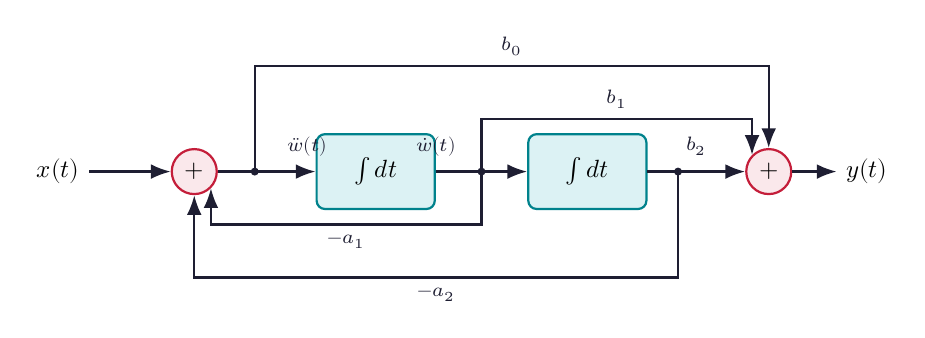
\begin{tikzpicture}[>=Latex, font=\small, scale=0.96]
  % Input and first summer
  \node (x) at (-0.6, 0) {$x(t)$};
  \node[circnode, inner sep=2.5pt] (s1) at (1.2, 0) {$+$};
  \draw[arrowline] (x) -- (s1);

  % Central integrator chain
  \node[sysblock, minimum width=1.5cm, minimum height=0.95cm] (int1) at (3.6, 0) {$\int dt$};
  \node[sysblock, minimum width=1.5cm, minimum height=0.95cm] (int2) at (6.4, 0) {$\int dt$};
  \draw[arrowline] (s1) -- (int1);
  \node[above=2pt, font=\scriptsize, color=mydark] at (2.7, 0) {$\ddot{w}(t)$};
  \draw[arrowline] (int1) -- (int2);
  \node[above=2pt, font=\scriptsize, color=mydark] at (4.4, 0) {$\dot{w}(t)$};

  % Second summer and output
  \node[circnode, inner sep=2.5pt] (s2) at (8.8, 0) {$+$};
  \node (y) at (10.1, 0) {$y(t)$};
  \draw[arrowline] (s2) -- (y);
  \draw[arrowline] (int2) -- node[above=2pt, font=\scriptsize] {$b_2$} (s2);

  % Branch point 1: w''(t)
  \coordinate (br0) at (2.0, 0);
  \fill[mydark] (br0) circle (1.5pt);
  % Direct feedthrough b0 (high top arch to s2.north)
  \draw[arrowline] (br0) -- ++(0, 1.4) -| node[pos=0.25, above, font=\scriptsize] {$b_0$} (s2.north);

  % Branch point 2: w'(t)
  \coordinate (br1) at (5.0, 0);
  \fill[mydark] (br1) circle (1.5pt);
  % Forward path b1 (medium top arch to s2.north west)
  \draw[arrowline] (br1) -- ++(0, 0.7) -| node[pos=0.25, above, font=\scriptsize] {$b_1$} (s2.north west);
  % Feedback path -a1 (medium bottom arch to s1.south east)
  \draw[arrowline] (br1) -- ++(0, -0.7) -| node[pos=0.25, below, font=\scriptsize] {$-a_1$} (s1.south east);

  % Branch point 3: w(t)
  \coordinate (br2) at (7.6, 0);
  \fill[mydark] (br2) circle (1.5pt);
  % Feedback path -a2 (low bottom arch to s1.south)
  \draw[arrowline] (br2) -- ++(0, -1.4) -| node[pos=0.25, below, font=\scriptsize] {$-a_2$} (s1.south);
\end{tikzpicture}
\end{center}
\end{tcolorbox}

% ───────────────────────────────────────────────────────────────────────────────
\section{Behavior with Aperiodic Convergent Inputs}
% ───────────────────────────────────────────────────────────────────────────────

When an aperiodic convergent input signal (such as an exponentially decaying signal $x(t) = e^{-at}u(t)$, $a > 0$) is applied to an LSI system:
\begin{itemize}[topsep=2pt, itemsep=2pt]
  \item \textbf{Energy Preservation:} If both $x(t)$ and $h(t)$ are $L_1$ and $L_2$ bounded (energy signals), the output $y(t) = x(t) * h(t)$ is also guaranteed to be an energy signal:
  \begin{equation}
    E_y = \int_{-\infty}^{\infty} |y(t)|^2 dt < \infty
  \end{equation}
  \item \textbf{Convergence to Zero:} Since $\lim_{t \to \infty} x(t) = 0$, for any stable system with $\int |h(t)|dt < \infty$, the output asymptotically decays to zero:
  \begin{equation}
    \lim_{t \to \infty} y(t) = \lim_{t \to \infty} \int_0^t x(\tau) h(t - \tau) d\tau = 0
  \end{equation}
  \item \textbf{Transient Decay Rate:} The overall decay envelope is governed by the slowest pole (dominant time constant) among the system and the input excitation.
\end{itemize}

% ───────────────────────────────────────────────────────────────────────────────
% QUICK REVISION PAGE
% ───────────────────────────────────────────────────────────────────────────────
\newpage
\begin{center}
  {\Large\bfseries\color{myred} Quick Revision \& Examination Compendium}\\[3pt]
  {\small\color{watermark}\textbf{Module 2: Linear Shift-Invariant Systems \& Convolution}}
\end{center}
\vspace{-2pt}
\noindent{\color{myred}\rule{\linewidth}{0.8pt}}

\begin{tcolorbox}[formulabox, title={\textbf{Key Formulas at a Glance}}]
\par\vspace{4pt}\noindent
\begingroup
\setlength{\tabcolsep}{5pt}
\setlength{\extrarowheight}{3pt}
\renewcommand{\arraystretch}{1.4}
\begin{tabularx}{\linewidth}{|B{4.5cm}|Y|}
\hline
\textbf{Concept / Law} & \textbf{Mathematical Equation} \\
\hline
Continuous-Time Convolution & $y(t) = x(t) * h(t) = \int_{-\infty}^{\infty} x(\tau) h(t - \tau) d\tau$ \\
\hline
Discrete-Time Convolution & $y[n] = x[n] * h[n] = \sum_{k=-\infty}^{\infty} x[k] h[n - k]$ \\
\hline
Step Response from Impulse & $s(t) = \int_{-\infty}^t h(\tau) d\tau, \quad s[n] = \sum_{k=-\infty}^n h[k]$ \\
\hline
Impulse Response from Step & $h(t) = \frac{ds(t)}{dt}, \quad h[n] = s[n] - s[n-1]$ \\
\hline
LTI Causality Condition & $h(t) = 0 \quad \forall t < 0, \qquad h[n] = 0 \quad \forall n < 0$ \\
\hline
LTI BIBO Stability Condition & $\int_{-\infty}^{\infty} |h(t)| dt < \infty, \qquad \sum_{n=-\infty}^{\infty} |h[n]| < \infty$ \\
\hline
Cascade Connection & $h_{eq}(t) = h_1(t) * h_2(t) = h_2(t) * h_1(t)$ \\
\hline
Parallel Connection & $h_{eq}(t) = h_1(t) + h_2(t)$ \\
\hline
Convolution with Shifted Impulse & $x(t) * \delta(t - t_0) = x(t - t_0)$ \\
\hline
LCCDE Zero-State Output & $y_{zs}(t) = x(t) * h(t) \quad \text{under initial rest}$ \\
\hline
\end{tabularx}
\endgroup
\end{tcolorbox}

\begin{tcolorbox}[defbox, title={\textbf{One-Line Definitions for Rapid Review}}]
\par\vspace{4pt}\noindent
\begingroup
\setlength{\tabcolsep}{5pt}
\setlength{\extrarowheight}{3pt}
\renewcommand{\arraystretch}{1.35}
\begin{tabularx}{\linewidth}{|B{4.2cm}|Y|}
\hline
\textbf{Term} & \textbf{Definitive Technical Meaning} \\
\hline
Impulse Response $h(t)$ & The output response of an LTI system when excited by a unit impulse under zero initial conditions. \\
\hline
Step Response $s(t)$ & The response of an LTI system to a unit step input under initial rest conditions. \\
\hline
Convolution & A mathematical operator combining two signals to express how the shape of one is modified by the other. \\
\hline
Initial Rest & The condition where a system has zero internal energy stored prior to the instant an input is applied. \\
\hline
Causal LSI System & An LTI system whose impulse response is strictly zero for all negative time ($h(t) = 0, t < 0$). \\
\hline
BIBO Stable LSI System & An LTI system whose impulse response is absolutely integrable ($\int |h(t)|dt < \infty$). \\
\hline
Zero-Input Response (ZIR) & The system output generated solely by non-zero initial states in the absence of any input. \\
\hline
Zero-State Response (ZSR) & The system output generated solely by the external input when all initial states are zero. \\
\hline
Canonic Realization & A block diagram realization containing the minimum possible number of delay or integrator elements ($N$). \\
\hline
\end{tabularx}
\endgroup
\end{tcolorbox}

\begin{tcolorbox}[exambox, title={\textbf{Frequently Asked / Viva Questions}}]
\begin{enumerate}[topsep=0pt, label=\textbf{Q\arabic*.}, itemsep=5pt]
  \item \Q{Why does the impulse response $h(t)$ completely characterize an LSI system?}
  Because any input $x(t)$ can be represented as an integral of weighted, shifted impulses. By linearity (superposition) and time-invariance, the output is the corresponding integral of weighted, shifted impulse responses. Thus, knowing $h(t)$ determines the response to \textit{any} arbitrary input.

  \item \Q{How can you compute the impulse response if the step response is known?}
  For continuous-time systems, differentiate the step response: $h(t) = \frac{ds(t)}{dt}$. For discrete-time systems, take the first backward difference: $h[n] = s[n] - s[n-1]$.

  \item \Q{Prove that convolution is commutative: $x(t) * h(t) = h(t) * x(t)$.}
  By definition, $x(t) * h(t) = \int_{-\infty}^{\infty} x(\tau) h(t - \tau) d\tau$. Substituting $v = t - \tau \implies d\tau = -dv$. When $\tau = -\infty, v = +\infty$; when $\tau = +\infty, v = -\infty$. Thus:
  $\int_{+\infty}^{-\infty} x(t - v) h(v) (-dv) = \int_{-\infty}^{\infty} h(v) x(t - v) dv = h(t) * x(t)$.

  \item \Q{What is the total duration of the convolution of two signals of lengths $T_1$ and $T_2$?}
  In continuous-time, the duration is $T_1 + T_2$. In discrete-time, if signal 1 has $N_1$ samples and signal 2 has $N_2$ samples, the convolved output has exactly $N_1 + N_2 - 1$ samples.

  \item \Q{State the necessary and sufficient condition for an LSI system to be causal.}
  The impulse response must be zero for all negative time: $h(t) = 0$ for $t < 0$ (or $h[n] = 0$ for $n < 0$).

  \item \Q{Is the system with impulse response $h(t) = e^{2t} u(t)$ stable? Why?}
  No. Evaluating absolute integrability: $\int_{-\infty}^\infty |h(t)|dt = \int_0^\infty e^{2t} dt = \left[\frac{e^{2t}}{2}\right]_0^\infty = \infty$. Since it is not absolutely integrable, it is BIBO unstable.

  \item \Q{What is the difference between Zero-Input Response (ZIR) and Zero-State Response (ZSR)?}
  ZIR is driven purely by initial energy/conditions stored in capacitors/inductors with zero external input. ZSR is driven purely by the applied input with zero initial stored energy. Total response is $y(t) = y_{zir}(t) + y_{zsr}(t)$.

  \item \Q{Why does the condition of initial rest ensure that a differential equation represents an LTI system?}
  Non-zero initial conditions introduce an additive constant independent of the input, violating linearity (homogeneity $y(0) \ne 0$) and causing time-variant behavior. Initial rest enforces zero state prior to excitation, ensuring linearity, time-invariance, and causality.

  \item \Q{Why are integrators preferred over differentiators in analog computer simulation of LCCDE?}
  Differentiators have transfer function $s$, which amplifies high-frequency noise and introduces signal instability. Integrators have transfer function $1/s$, which attenuates high frequencies, acting as low-pass filters that provide stable, noise-free computation.

  \item \Q{What is the convolution of a signal $x(t)$ with a unit step $u(t)$?}
  $x(t) * u(t) = \int_{-\infty}^\infty x(\tau) u(t - \tau) d\tau = \int_{-\infty}^t x(\tau) d\tau$. Convolution with a unit step is equivalent to running integration of the signal from $-\infty$ to $t$.
\end{enumerate}
\end{tcolorbox}

\begin{tcolorbox}[tikzbox, title={\textbf{Summary Matrix: LSI Characterization Across Domains}}]
\par\vspace{4pt}\noindent
\begingroup
\setlength{\tabcolsep}{4.5pt}
\setlength{\extrarowheight}{3pt}
\renewcommand{\arraystretch}{1.35}
\begin{tabularx}{\linewidth}{|B{3.2cm}|B{4.5cm}|Y|}
\hline
\textbf{Property} & \textbf{Continuous-Time (CT)} & \textbf{Discrete-Time (DT)} \\
\hline
Impulse Input & Dirac Delta $\delta(t)$ & Kronecker Delta $\delta[n]$ \\
\hline
Convolution & $y(t) = \int_{-\infty}^\infty x(\tau) h(t-\tau) d\tau$ & $y[n] = \sum_{k=-\infty}^\infty x[k] h[n-k]$ \\
\hline
Causality & $h(t) = 0 \quad \forall t < 0$ & $h[n] = 0 \quad \forall n < 0$ \\
\hline
BIBO Stability & $\int_{-\infty}^\infty |h(t)| dt < \infty$ & $\sum_{n=-\infty}^\infty |h[n]| < \infty$ \\
\hline
Step Response $s$ & $s(t) = \int_{-\infty}^t h(\tau) d\tau$ & $s[n] = \sum_{k=-\infty}^n h[k]$ \\
\hline
Recovery of $h$ & $h(t) = \frac{ds(t)}{dt}$ & $h[n] = s[n] - s[n-1]$ \\
\hline
Interconnection & Cascade: $h_1 * h_2$; Parallel: $h_1 + h_2$ & Cascade: $h_1 * h_2$; Parallel: $h_1 + h_2$ \\
\hline
\end{tabularx}
\endgroup
\end{tcolorbox}


% -- Module 3 -----------------------------------------------------------------
\modulestart{3}{Eigenfunctions and Periodic Inputs to LSI Systems}

\section{Eigenfunctions and Periodic Inputs to LSI Systems}
% ───────────────────────────────────────────────────────────────────────────────

\subsection{Eigenfunctions of Continuous-Time LSI Systems}

\begin{tcolorbox}[defbox, title={\textbf{Definition: Eigenfunction of an LSI System}}]
An input signal $x(t)$ is termed an \textbf{eigenfunction} of an LSI system $\mathcal{T}$ if the resulting output $y(t)$ is simply a scaled replica of the same input signal:
\begin{equation}
  y(t) = \mathcal{T}\{x(t)\} = \lambda \cdot x(t)
\end{equation}
where the complex scalar $\lambda \in \mathbb{C}$ is the corresponding \textbf{eigenvalue}.
\end{tcolorbox}

\textbf{Proof that Complex Exponentials are Eigenfunctions:}
Let the input to a continuous-time LSI system with impulse response $h(t)$ be the complex exponential $x(t) = e^{s t}$, where $s = \sigma + j\omega \in \mathbb{C}$. By the convolution integral:
\begin{align}
  y(t) &= \int_{-\infty}^{\infty} h(\tau) x(t - \tau) d\tau = \int_{-\infty}^{\infty} h(\tau) e^{s(t - \tau)} d\tau \\
  &= e^{st} \left[ \int_{-\infty}^{\infty} h(\tau) e^{-s\tau} d\tau \right]
\end{align}
Notice that the bracketed integral is purely a function of the complex frequency variable $s$, independent of time $t$. Defining the system transfer function $H(s) \triangleq \int_{-\infty}^\infty h(\tau) e^{-s\tau} d\tau$:
\begin{equation}
  y(t) = H(s) \cdot e^{st}
\end{equation}
For purely imaginary frequencies $s = j\omega$, the input is the harmonic phasor $x(t) = e^{j\omega t}$, yielding:
\begin{equation}
  y(t) = H(j\omega) \cdot e^{j\omega t}
\end{equation}
Thus, \textbf{complex exponentials are eigenfunctions of LSI systems}, and the corresponding eigenvalue is the system's \textbf{Frequency Response} $H(j\omega)$.

\subsection{Response to Periodic and Semi-Periodic Inputs}
By the principle of superposition, if a periodic input is decomposed into a sum of harmonically related complex exponentials:
\begin{equation}
  x(t) = \sum_{k=-\infty}^{\infty} c_k e^{j k \omega_0 t}
\end{equation}
The steady-state response of the LSI system is directly obtained by scaling each harmonic component by the frequency response evaluated at that specific harmonic:
\begin{equation}
  y(t) = \sum_{k=-\infty}^{\infty} c_k H(j k \omega_0) e^{j k \omega_0 t}
\end{equation}

\textbf{Semi-Periodic Inputs:}
A semi-periodic signal is one that is periodic for $t \ge 0$ but zero for $t < 0$, represented as $x(t) = p(t) u(t)$, where $p(t + T_0) = p(t)$. When applied to an LSI system:
\begin{itemize}[topsep=2pt, itemsep=2pt]
  \item The total response consists of a \textbf{transient response} $y_{tr}(t)$ and a \textbf{steady-state response} $y_{ss}(t)$:
  \begin{equation}
    y(t) = y_{tr}(t) + y_{ss}(t)
  \end{equation}
  \item For a BIBO stable system, the transient response decays exponentially to zero ($\lim_{t\to\infty} y_{tr}(t) = 0$), and the output asymptotically converges to the purely periodic steady-state response $y_{ss}(t)$.
\end{itemize}

% ───────────────────────────────────────────────────────────────────────────────
\section{The Frequency Response \texorpdfstring{$H(j\omega)$}{H(j omega)}}
% ───────────────────────────────────────────────────────────────────────────────

\subsection{Definition and Relation to Impulse Response}

\begin{tcolorbox}[defbox, title={\textbf{Definition: Frequency Response}}]
The \textbf{Frequency Response} $H(j\omega)$ of a continuous-time LSI system is the Continuous-Time Fourier Transform (CTFT) of its unit impulse response $h(t)$:
\begin{equation}
  H(j\omega) \triangleq \mathcal{F}\{h(t)\} = \int_{-\infty}^{\infty} h(t) e^{-j\omega t} dt
\end{equation}
Conversely, the impulse response is recovered via the Inverse Fourier Transform:
\begin{equation}
  h(t) = \frac{1}{2\pi} \int_{-\infty}^{\infty} H(j\omega) e^{j\omega t} d\omega
\end{equation}
\end{tcolorbox}

\subsection{Magnitude Response and Phase Response}
In polar form, $H(j\omega)$ is expressed as:
\begin{equation}
  H(j\omega) = |H(j\omega)| e^{j \angle H(j\omega)}
\end{equation}
where:
\begin{itemize}[topsep=2pt, itemsep=2pt]
  \item $|H(j\omega)|$ is the \textbf{Magnitude Response} (or amplitude gain) of the system at frequency $\omega$.
  \item $\angle H(j\omega) = \arg[H(j\omega)]$ is the \textbf{Phase Response} (phase shift) imparted to the input phasor.
  \item \textbf{Group Delay $\tau_g(\omega)$:} The time delay experienced by a narrow-band signal envelope centered at frequency $\omega$:
  \begin{equation}
    \tau_g(\omega) \triangleq -\frac{d}{d\omega} \angle H(j\omega)
  \end{equation}
\end{itemize}

\textbf{Symmetry Properties for Real Impulse Response $h(t) \in \mathbb{R}$:}
\begin{enumerate}[topsep=2pt, itemsep=2pt]
  \item Conjugate symmetry: $H(-j\omega) = H^*(j\omega)$.
  \item Even magnitude symmetry: $|H(-j\omega)| = |H(j\omega)|$.
  \item Odd phase symmetry: $\angle H(-j\omega) = -\angle H(j\omega)$.
\end{enumerate}

\begin{tcolorbox}[examplebox, title={\textbf{Sinusoidal Steady-State Response}}]
If the input to an LSI system is a real sinusoid $x(t) = A \cos(\omega_0 t + \theta)$, the steady-state output is:
\begin{equation}
  y(t) = A |H(j\omega_0)| \cos\big(\omega_0 t + \theta + \angle H(j\omega_0)\big)
\end{equation}
The frequency remains completely unchanged; the system only scales the amplitude by $|H(j\omega_0)|$ and shifts the phase by $\angle H(j\omega_0)$.
\end{tcolorbox}

% ───────────────────────────────────────────────────────────────────────────────
\section{Continuous-Time Fourier Series (CTFS)}
% ───────────────────────────────────────────────────────────────────────────────

\subsection{Dirichlet Conditions for Convergence}
A periodic signal $x(t)$ with fundamental period $T_0$ and fundamental frequency $\omega_0 = 2\pi / T_0$ can be expanded in a Fourier series if it satisfies the \textbf{Dirichlet Conditions}:
\begin{enumerate}[topsep=2pt, itemsep=2pt]
  \item \textbf{Absolute Integrability:} Over any single period $T_0$, $\int_{T_0} |x(t)| dt < \infty$.
  \item \textbf{Bounded Variation:} $x(t)$ has a finite number of local maxima and minima within any single period.
  \item \textbf{Finite Discontinuities:} $x(t)$ has a finite number of discontinuities within any period, and each discontinuity is finite (bounded jump).
\end{enumerate}
At a point of finite discontinuity $t_0$, the Fourier series converges to the arithmetic mean of the left- and right-hand limits: $\frac{x(t_0^+) + x(t_0^-)}{2}$.

\subsection{Three Formulations of Fourier Series}

\par\vspace{6pt}\noindent
\begingroup
\setlength{\tabcolsep}{5pt}
\setlength{\extrarowheight}{3pt}
\renewcommand{\arraystretch}{1.4}
\begin{tabularx}{\linewidth}{|B{4cm}|Y|Y|}
\hline
\textbf{Representation} & \textbf{Synthesis Equation} & \textbf{Analysis / Coefficient Equations} \\
\hline
Trigonometric Fourier Series (TFS) & $x(t) = a_0 + \sum_{n=1}^\infty [a_n \cos(n\omega_0 t) + b_n \sin(n\omega_0 t)]$ & $a_0 = \frac{1}{T_0} \int_{T_0} x(t) dt$, \par $a_n = \frac{2}{T_0} \int_{T_0} x(t) \cos(n\omega_0 t) dt$, \par $b_n = \frac{2}{T_0} \int_{T_0} x(t) \sin(n\omega_0 t) dt$ \\
\hline
Compact / Polar Form & $x(t) = C_0 + \sum_{n=1}^\infty C_n \cos(n\omega_0 t + \theta_n)$ & $C_0 = a_0$, \quad $C_n = \sqrt{a_n^2 + b_n^2}$, \par $\theta_n = -\tan^{-1}(b_n / a_n)$ \\
\hline
Exponential / Complex Form (EFS) & $x(t) = \sum_{k=-\infty}^\infty c_k e^{j k \omega_0 t}$ & $c_k = \frac{1}{T_0} \int_{T_0} x(t) e^{-j k \omega_0 t} dt$ \\
\hline
\end{tabularx}
\endgroup

\subsection{Inter-Relationship Between TFS and EFS Coefficients}
\begin{align}
  c_0 &= a_0 = C_0 \\
  c_k &= \frac{a_k - j b_k}{2} = \frac{C_k}{2} e^{j\theta_k}, \qquad c_{-k} = c_k^* = \frac{a_k + j b_k}{2} = \frac{C_k}{2} e^{-j\theta_k} \\
  a_k &= c_k + c_{-k} = 2 \text{Re}\{c_k\}, \qquad b_k = j(c_k - c_{-k}) = -2 \text{Im}\{c_k\}
\end{align}

\subsection{Gibbs Phenomenon}
When a discontinuous signal (such as a square wave) is approximated by a truncated Fourier series with $N$ harmonics, an oscillatory overshoot occurs in the immediate vicinity of the discontinuity. As $N \to \infty$, the overshoot does not disappear; its width narrows to zero, but its peak amplitude approaches a fixed constant:
\begin{equation}
  \text{Overshoot Percentage} = \frac{\frac{2}{\pi} \int_0^\pi \frac{\sin x}{x} dx - 1}{1} \approx 8.95\% \approx 9\% \text{ of the jump discontinuity}
\end{equation}

% ───────────────────────────────────────────────────────────────────────────────
\section{Continuous-Time Fourier Transform (CTFT)}
% ───────────────────────────────────────────────────────────────────────────────

\subsection{Transition from Fourier Series to Fourier Transform}
An aperiodic signal $x(t)$ can be viewed as the limiting case of a periodic signal as the period $T_0 \to \infty$. In this limit:
\begin{itemize}[topsep=2pt, itemsep=2pt]
  \item The fundamental frequency $\omega_0 = 2\pi / T_0 \to d\omega$ becomes an infinitesimal differential.
  \item The discrete harmonic frequencies $k \omega_0 \to \omega$ merge into a continuous frequency continuum.
  \item The discrete spectrum $T_0 c_k$ transforms into the continuous spectral density $X(j\omega)$.
\end{itemize}

\begin{tcolorbox}[formulabox, title={\textbf{The Continuous-Time Fourier Transform (CTFT) Pair}}]
\begin{align}
  \textbf{Analysis (Forward CTFT):} \quad &X(j\omega) = \mathcal{F}\{x(t)\} = \int_{-\infty}^{\infty} x(t) e^{-j\omega t} dt \\
  \textbf{Synthesis (Inverse CTFT):} \quad &x(t) = \mathcal{F}^{-1}\{X(j\omega)\} = \frac{1}{2\pi} \int_{-\infty}^{\infty} X(j\omega) e^{j\omega t} d\omega
\end{align}
\end{tcolorbox}

\subsection{Properties of CTFT}

\par\vspace{6pt}\noindent
\begingroup
\setlength{\tabcolsep}{5pt}
\setlength{\extrarowheight}{3pt}
\renewcommand{\arraystretch}{1.4}
\begin{tabularx}{\linewidth}{|B{3.8cm}|B{4.5cm}|Y|}
\hline
\textbf{Property} & \textbf{Time Domain $x(t)$} & \textbf{Frequency Domain $X(j\omega)$} \\
\hline
Linearity & $a x_1(t) + b x_2(t)$ & $a X_1(j\omega) + b X_2(j\omega)$ \\
\hline
Time Shifting & $x(t - t_0)$ & $X(j\omega) e^{-j\omega t_0}$ \\
\hline
Frequency Shifting (Modulation) & $x(t) e^{j\omega_0 t}$ & $X(j(\omega - \omega_0))$ \\
\hline
Time Scaling & $x(at) \quad (a \ne 0)$ & $\frac{1}{|a|} X\left(j\frac{\omega}{a}\right)$ \\
\hline
Time Reversal & $x(-t)$ & $X(-j\omega) = X^*(j\omega) \quad (\text{if } x(t)\in\mathbb{R})$ \\
\hline
Duality & $X(jt)$ & $2\pi x(-\omega)$ \\
\hline
Time Differentiation & $\frac{d^n x(t)}{dt^n}$ & $(j\omega)^n X(j\omega)$ \\
\hline
Time Integration & $\int_{-\infty}^t x(\tau) d\tau$ & $\frac{1}{j\omega} X(j\omega) + \pi X(0) \delta(\omega)$ \\
\hline
Time Convolution & $x_1(t) * x_2(t)$ & $X_1(j\omega) \cdot X_2(j\omega)$ \\
\hline
Frequency Convolution (Multiplication) & $x_1(t) \cdot x_2(t)$ & $\frac{1}{2\pi} \big[ X_1(j\omega) * X_2(j\omega) \big]$ \\
\hline
\end{tabularx}
\endgroup

\subsection{Fourier Domain Duality}
The mathematical symmetry between the analysis and synthesis integrals leads to the \textbf{Duality Property}:
\begin{equation}
  \text{If } \mathcal{F}\{x(t)\} = X(j\omega), \quad \text{then } \mathcal{F}\{X(jt)\} = 2\pi x(-\omega)
\end{equation}
\textbf{Example:} Since a rectangular pulse in time transforms into a sinc function in frequency:
\begin{equation}
  \text{rect}\left(\frac{t}{\tau}\right) \iff \tau \text{sinc}\left(\frac{\omega\tau}{2\pi}\right)
\end{equation}
By duality, a sinc pulse in time transforms into an ideal rectangular spectrum in frequency:
\begin{equation}
  W \text{sinc}\left(\frac{Wt}{2\pi}\right) \iff 2\pi \cdot \text{rect}\left(\frac{\omega}{W}\right)
\end{equation}
This establishes that ideal bandlimited filtering in frequency corresponds to infinite sinc impulse responses in time.

% ───────────────────────────────────────────────────────────────────────────────
\section{Parseval's Theorem and Energy Spectral Density}
% ───────────────────────────────────────────────────────────────────────────────

\begin{tcolorbox}[formulabox, title={\textbf{Parseval's Energy Theorem}}]
\textbf{For Continuous-Time Fourier Transform:}
Total signal energy $E$ calculated in the time domain equals the energy integrated across all frequencies:
\begin{equation}
  E = \int_{-\infty}^{\infty} |x(t)|^2 dt = \frac{1}{2\pi} \int_{-\infty}^{\infty} |X(j\omega)|^2 d\omega = \int_{-\infty}^{\infty} |X(f)|^2 df
\end{equation}
where $f = \omega / 2\pi$ is frequency in Hertz.

\textbf{For Periodic Signals (CTFS):}
The average power $P$ equals the sum of the average powers in all individual harmonic components:
\begin{equation}
  P = \frac{1}{T_0} \int_{T_0} |x(t)|^2 dt = \sum_{k=-\infty}^{\infty} |c_k|^2 = C_0^2 + \frac{1}{2}\sum_{n=1}^{\infty} C_n^2
\end{equation}
\end{tcolorbox}

\textbf{Energy Spectral Density (ESD):}
The quantity $S_{xx}(\omega) \triangleq |X(j\omega)|^2$ represents the distribution of energy per unit frequency (in Joules/(rad/s)). When a signal passes through an LSI system:
\begin{equation}
  Y(j\omega) = X(j\omega) H(j\omega) \implies S_{yy}(\omega) = |Y(j\omega)|^2 = |H(j\omega)|^2 S_{xx}(\omega)
\end{equation}

% ───────────────────────────────────────────────────────────────────────────────
\section{Discrete-Time Fourier Transform (DTFT) \& Discrete Fourier Transform (DFT)}
% ───────────────────────────────────────────────────────────────────────────────

\subsection{Discrete-Time Fourier Transform (DTFT)}
The DTFT applies to infinite-length discrete-time sequences $x[n]$.

\begin{tcolorbox}[defbox, title={\textbf{Definition: DTFT and Inverse DTFT}}]
\begin{align}
  \textbf{Forward DTFT (Analysis):} \quad &X(e^{j\Omega}) = \sum_{n=-\infty}^{\infty} x[n] e^{-j\Omega n} \\
  \textbf{Inverse DTFT (Synthesis):} \quad &x[n] = \frac{1}{2\pi} \int_{-\pi}^{\pi} X(e^{j\Omega}) e^{j\Omega n} d\Omega
\end{align}
\end{tcolorbox}

\textbf{Fundamental Property: $2\pi$-Periodicity in Frequency:}
Since $e^{-j(\Omega + 2\pi) n} = e^{-j\Omega n} e^{-j 2\pi n} = e^{-j\Omega n} \cdot 1$:
\begin{equation}
  X(e^{j(\Omega + 2\pi)}) = X(e^{j\Omega})
\end{equation}
All distinct frequency information is fully contained within any interval of length $2\pi$, conventionally chosen as $[-\pi, \pi]$ or $[0, 2\pi]$.

\subsection{Discrete Fourier Transform (DFT)}
The DFT operates on finite-duration discrete-time sequences of length $N$, producing an $N$-point discrete frequency spectrum suitable for digital computer computation.

\begin{tcolorbox}[defbox, title={\textbf{Definition: Discrete Fourier Transform (DFT) Pair}}]
Let $x[n]$ be an $N$-point sequence defined for $n = 0, 1, \dots, N-1$.
\begin{align}
  \textbf{DFT (Analysis):} \quad &X[k] = \sum_{n=0}^{N-1} x[n] W_N^{kn}, \qquad k = 0, 1, \dots, N-1 \\
  \textbf{IDFT (Synthesis):} \quad &x[n] = \frac{1}{N} \sum_{k=0}^{N-1} X[k] W_N^{-kn}, \qquad n = 0, 1, \dots, N-1
\end{align}
where the \textbf{Twiddle Factor} is $W_N \triangleq e^{-j\frac{2\pi}{N}}$.
\end{tcolorbox}

\subsection{Relation Between DTFT and DFT}
The DFT values $X[k]$ are exact samples of the continuous DTFT $X(e^{j\Omega})$ evaluated at $N$ uniformly spaced points along the unit circle:
\begin{equation}
  X[k] = \left. X(e^{j\Omega}) \right|_{\Omega = \frac{2\pi k}{N}}, \qquad k = 0, 1, \dots, N-1
\end{equation}

% ───────────────────────────────────────────────────────────────────────────────
\section{Signal Space and Orthogonal Bases}
% ───────────────────────────────────────────────────────────────────────────────

\subsection{The Signal Space Concept (Hilbert Space $L^2$)}
Signals can be viewed as vectors residing in an infinite-dimensional vector space known as a \textbf{Hilbert Space} $\mathcal{H} = L^2[a,b]$. The geometric concepts of length, distance, and angle in Euclidean space generalize directly to signals:

\begin{itemize}[topsep=2pt, itemsep=2pt]
  \item \textbf{Inner Product $\langle x, y \rangle$:} The inner product of two signals $x(t)$ and $y(t)$ over interval $[t_1, t_2]$ is:
  \begin{equation}
    \langle x, y \rangle \triangleq \int_{t_1}^{t_2} x(t) y^*(t) dt
  \end{equation}
  \item \textbf{Signal Norm (Magnitude/Length):} The norm $\|x\|$ is defined as:
  \begin{equation}
    \|x\| \triangleq \sqrt{\langle x, x \rangle} = \left[ \int_{t_1}^{t_2} |x(t)|^2 dt \right]^{1/2} = \sqrt{E_x}
  \end{equation}
  where $E_x$ is the total energy of the signal.
  \item \textbf{Metric (Distance between Signals):} $d(x, y) = \|x - y\| = \sqrt{\int_{t_1}^{t_2} |x(t) - y(t)|^2 dt}$.
\end{itemize}

\subsection{Orthogonality and Orthonormal Bases}

\begin{tcolorbox}[defbox, title={\textbf{Definition: Orthogonal and Orthonormal Signal Sets}}]
A set of basis functions $\{\phi_1(t), \phi_2(t), \dots, \phi_N(t)\}$ is:
\begin{enumerate}[topsep=2pt, itemsep=2pt]
  \item \textbf{Orthogonal} if the inner product of distinct basis functions is strictly zero:
  \begin{equation}
    \langle \phi_i, \phi_j \rangle = \int_{t_1}^{t_2} \phi_i(t) \phi_j^*(t) dt = \begin{cases} 0, & i \ne j \\ E_i \ne 0, & i = j \end{cases}
  \end{equation}
  \item \textbf{Orthonormal} if it is orthogonal and every basis function has unit energy ($E_i = 1$):
  \begin{equation}
    \langle \phi_i, \phi_j \rangle = \delta_{ij} = \begin{cases} 1, & i = j \\ 0, & i \ne j \end{cases}
  \end{equation}
  where $\delta_{ij}$ is the Kronecker delta.
\end{enumerate}
\end{tcolorbox}

\subsection{Generalized Fourier Series Expansion}
Any arbitrary signal $x(t) \in \mathcal{H}$ can be represented as a linear combination of orthonormal basis functions:
\begin{equation}
  x(t) = \sum_{k=1}^{\infty} c_k \phi_k(t)
\end{equation}
Taking the inner product of both sides with $\phi_m(t)$:
\begin{equation}
  \langle x, \phi_m \rangle = \left\langle \sum_{k=1}^{\infty} c_k \phi_k, \phi_m \right\rangle = \sum_{k=1}^{\infty} c_k \langle \phi_k, \phi_m \rangle = \sum_{k=1}^{\infty} c_k \delta_{km} = c_m
\end{equation}
Hence, the projection coefficients are given by the projection integral:
\begin{equation}
  c_k = \langle x, \phi_k \rangle = \int_{t_1}^{t_2} x(t) \phi_k^*(t) dt
\end{equation}

\textbf{Generalized Parseval's Identity:}
If the basis $\{\phi_k(t)\}$ is complete:
\begin{equation}
  \|x\|^2 = \int_{t_1}^{t_2} |x(t)|^2 dt = \sum_{k=1}^{\infty} |c_k|^2
\end{equation}
The continuous-time Exponential Fourier Series is simply a special case where the orthonormal basis is $\phi_k(t) = \frac{1}{\sqrt{T_0}} e^{j k \omega_0 t}$ over interval $[0, T_0]$.

\begin{tcolorbox}[tikzbox, title={\textbf{TikZ Illustration: Signal Projection onto Orthogonal Basis Axes}}]
\begin{center}
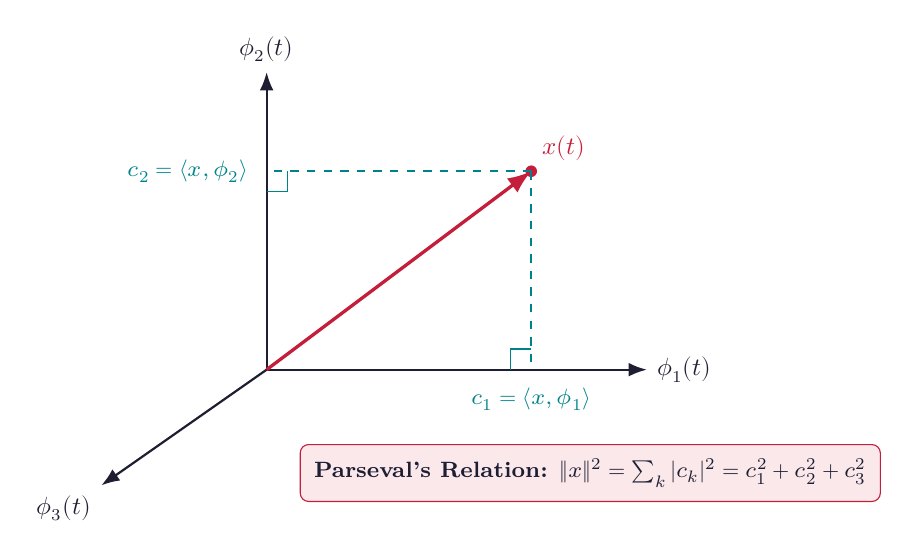
\begin{tikzpicture}[>=Latex, scale=1.05, font=\small]
  % Orthogonal Axes
  \draw[->, thick, color=mydark] (0,0) -- (4.6,0) node[right, font=\small\bfseries] {$\phi_1(t)$};
  \draw[->, thick, color=mydark] (0,0) -- (0,3.6) node[above, font=\small\bfseries] {$\phi_2(t)$};
  \draw[->, thick, color=mydark] (0,0) -- (-2.0,-1.4) node[below left, font=\small\bfseries] {$\phi_3(t)$};

  % Signal vector x(t)
  \draw[very thick, myred, -{Latex[length=3mm]}] (0,0) -- (3.2, 2.4) node[above right, font=\small\bfseries, color=myred] {$x(t)$};
  \fill[myred] (3.2, 2.4) circle (2pt);

  % Orthogonal Projections
  \draw[dashed, myteal, thick] (3.2, 2.4) -- (3.2, 0) node[below=3pt, color=myteal, font=\footnotesize\bfseries] {$c_1 = \langle x, \phi_1 \rangle$};
  \draw[dashed, myteal, thick] (3.2, 2.4) -- (0, 2.4) node[left=3pt, color=myteal, font=\footnotesize\bfseries] {$c_2 = \langle x, \phi_2 \rangle$};

  % Right angle indicator
  \draw[myteal] (3.2, 0.25) -- (2.95, 0.25) -- (2.95, 0);
  \draw[myteal] (0.25, 2.4) -- (0.25, 2.15) -- (0, 2.15);

  % Energy Formulation Box (Parseval's relation)
  \node[draw=myred, fill=hdrred, rounded corners=3pt, inner sep=5pt, font=\footnotesize\bfseries, text=mydark, anchor=west] at (0.4, -1.25) {
    Parseval's Relation: $\|x\|^2 = \sum_{k} |c_k|^2 = c_1^2 + c_2^2 + c_3^2$
  };
\end{tikzpicture}
\end{center}
\end{tcolorbox}

% ───────────────────────────────────────────────────────────────────────────────
% QUICK REVISION PAGE
% ───────────────────────────────────────────────────────────────────────────────
\newpage
\begin{center}
  {\Large\bfseries\color{myred} Quick Revision \& Examination Compendium}\\[3pt]
  {\small\color{watermark}\textbf{Module 3: Fourier Analysis, Frequency Response \& Signal Space}}
\end{center}
\vspace{-2pt}
\noindent{\color{myred}\rule{\linewidth}{0.8pt}}

\begin{tcolorbox}[formulabox, title={\textbf{Key Formulas at a Glance}}]
\par\vspace{4pt}\noindent
\begingroup
\setlength{\tabcolsep}{5pt}
\setlength{\extrarowheight}{3pt}
\renewcommand{\arraystretch}{1.4}
\begin{tabularx}{\linewidth}{|B{4.5cm}|Y|}
\hline
\textbf{Transform / Theorem} & \textbf{Definitive Mathematical Formula} \\
\hline
Frequency Response $H(j\omega)$ & $H(j\omega) = \int_{-\infty}^{\infty} h(t) e^{-j\omega t} dt = |H(j\omega)| e^{j\angle H(j\omega)}$ \\
\hline
Group Delay $\tau_g(\omega)$ & $\tau_g(\omega) = -\frac{d}{d\omega} \angle H(j\omega)$ \\
\hline
Exponential Fourier Series & $x(t) = \sum_{k=-\infty}^\infty c_k e^{j k \omega_0 t}, \quad c_k = \frac{1}{T_0} \int_{T_0} x(t) e^{-j k \omega_0 t} dt$ \\
\hline
CTFT Analysis / Synthesis & $X(j\omega) = \int_{-\infty}^\infty x(t) e^{-j\omega t} dt, \quad x(t) = \frac{1}{2\pi}\int_{-\infty}^\infty X(j\omega) e^{j\omega t} d\omega$ \\
\hline
CTFT Duality Property & $\mathcal{F}\{X(jt)\} = 2\pi x(-\omega)$ \\
\hline
CTFT Convolution & $\mathcal{F}\{x_1(t) * x_2(t)\} = X_1(j\omega) \cdot X_2(j\omega)$ \\
\hline
CTFT Multiplication & $\mathcal{F}\{x_1(t) \cdot x_2(t)\} = \frac{1}{2\pi} [X_1(j\omega) * X_2(j\omega)]$ \\
\hline
Parseval's Theorem (CTFT) & $\int_{-\infty}^\infty |x(t)|^2 dt = \frac{1}{2\pi} \int_{-\infty}^\infty |X(j\omega)|^2 d\omega$ \\
\hline
DTFT Analysis / Synthesis & $X(e^{j\Omega}) = \sum_n x[n] e^{-j\Omega n}, \quad x[n] = \frac{1}{2\pi}\int_{-\pi}^\pi X(e^{j\Omega}) e^{j\Omega n} d\Omega$ \\
\hline
DFT Analysis / Synthesis & $X[k] = \sum_{n=0}^{N-1} x[n] W_N^{kn}, \quad x[n] = \frac{1}{N} \sum_{k=0}^{N-1} X[k] W_N^{-kn}$ \\
\hline
Orthogonality Condition & $\langle \phi_i, \phi_j \rangle = \int \phi_i(t) \phi_j^*(t) dt = \delta_{ij} \|\phi_i\|^2$ \\
\hline
\end{tabularx}
\endgroup
\end{tcolorbox}

\begin{tcolorbox}[defbox, title={\textbf{One-Line Definitions for Rapid Review}}]
\par\vspace{4pt}\noindent
\begingroup
\setlength{\tabcolsep}{5pt}
\setlength{\extrarowheight}{3pt}
\renewcommand{\arraystretch}{1.35}
\begin{tabularx}{\linewidth}{|B{4.2cm}|Y|}
\hline
\textbf{Term} & \textbf{Definitive Technical Meaning} \\
\hline
Eigenfunction & A signal that when fed into an LSI system produces an output that is an exact scalar multiple of itself. \\
\hline
Frequency Response & The Fourier transform of the unit impulse response, expressing gain and phase shift vs frequency. \\
\hline
Group Delay & The negative derivative of phase with respect to angular frequency, indicating envelope propagation delay. \\
\hline
Dirichlet Conditions & Sufficient mathematical conditions (integrability, bounded extrema, finite jumps) for Fourier series convergence. \\
\hline
Gibbs Phenomenon & The persistent $\approx 9\%$ overshoot near step discontinuities in truncated Fourier series approximations. \\
\hline
Duality Property & The mathematical equivalence between time and frequency roles arising from symmetrical Fourier integrals. \\
\hline
Energy Spectral Density & The distribution of total signal energy as a function of continuous frequency, defined as $|X(j\omega)|^2$. \\
\hline
DTFT Periodicity & The inherent $2\pi$-periodicity of the discrete-time Fourier transform due to discrete sample spacing. \\
\hline
Twiddle Factor & The complex root of unity $W_N = e^{-j 2\pi / N}$ utilized in discrete Fourier transform calculations. \\
\hline
Hilbert Space & A complete vector space equipped with an inner product that defines length, distance, and angle for signals. \\
\hline
\end{tabularx}
\endgroup
\end{tcolorbox}

\begin{tcolorbox}[exambox, title={\textbf{Frequently Asked / Viva Questions}}]
\begin{enumerate}[topsep=0pt, label=\textbf{Q\arabic*.}, itemsep=5pt]
  \item \Q{Why are complex sinusoids $e^{j\omega t}$ eigenfunctions of continuous-time LSI systems?}
  When $e^{j\omega t}$ passes through an LSI system with impulse response $h(t)$, convolution gives $y(t) = \int h(\tau) e^{j\omega(t-\tau)} d\tau = e^{j\omega t} \int h(\tau) e^{-j\omega\tau} d\tau = H(j\omega) e^{j\omega t}$. The waveform shape is perfectly preserved; only its complex amplitude is scaled by eigenvalue $H(j\omega)$.

  \item \Q{What is the physical meaning of negative frequency $-\omega$ in Fourier analysis?}
  A complex phasor $e^{j\omega t}$ represents counter-clockwise rotation in the complex plane at angular speed $\omega$. A negative frequency $e^{-j\omega t}$ represents clockwise rotation at the same speed. In real sinusoids $\cos(\omega t) = \frac{e^{j\omega t} + e^{-j\omega t}}{2}$, positive and negative frequency phasors combine symmetrically to cancel imaginary components.

  \item \Q{State the relationship between time-domain convolution and frequency-domain multiplication.}
  Convolution in the time domain corresponds to pointwise multiplication in the frequency domain: $\mathcal{F}\{x(t) * h(t)\} = X(j\omega) \cdot H(j\omega)$. Conversely, multiplication in the time domain corresponds to convolution in the frequency domain: $\mathcal{F}\{x(t) \cdot p(t)\} = \frac{1}{2\pi} [X(j\omega) * P(j\omega)]$.

  \item \Q{What causes the Gibbs phenomenon and can it be eliminated by increasing harmonics?}
  Gibbs phenomenon is caused by non-uniform convergence of the Fourier series at jump discontinuities. Increasing the number of harmonics $N \to \infty$ narrows the spatial width of the ripple toward zero, but the peak amplitude remains fixed at approximately $8.95\%$ of the jump size. It can only be eliminated by windowing/smoothing techniques.

  \item \Q{How does the duality property allow you to find the Fourier transform of a sinc function?}
  Since a rectangular pulse in time $\text{rect}(t/\tau)$ transforms into $\tau \text{sinc}(\omega\tau/2\pi)$, applying duality ($\mathcal{F}\{X(jt)\} = 2\pi x(-\omega)$) reveals that a sinc pulse in time transforms into an ideal rectangular band in frequency.

  \item \Q{Why is the DTFT periodic with period $2\pi$ while the CTFT is non-periodic?}
  In discrete time, the sampling index $n$ is an integer. Thus, $e^{-j(\Omega + 2\pi)n} = e^{-j\Omega n} e^{-j 2\pi n} = e^{-j\Omega n} \cdot 1$. The basis functions themselves repeat every $2\pi$, forcing the DTFT $X(e^{j\Omega})$ to be strictly periodic with period $2\pi$.

  \item \Q{What is the key difference between DTFT and DFT?}
  DTFT operates on discrete sequences and yields a continuous, $2\pi$-periodic spectrum $X(e^{j\Omega})$. DFT operates on a finite sequence of $N$ points and yields $N$ discrete frequency samples $X[k]$, making DFT directly computable on digital hardware.

  \item \Q{What is the condition for two signals to be orthogonal over an interval $[t_1, t_2]$?}
  Two signals $x_1(t)$ and $x_2(t)$ are orthogonal if their inner product is zero: $\langle x_1, x_2 \rangle = \int_{t_1}^{t_2} x_1(t) x_2^*(t) dt = 0$.

  \item \Q{State Parseval's relation for energy signals and explain its conservation principle.}
  $\int_{-\infty}^{\infty} |x(t)|^2 dt = \frac{1}{2\pi} \int_{-\infty}^{\infty} |X(j\omega)|^2 d\omega$. It establishes that energy is conserved under the Fourier transformation: total energy computed across the entire time domain is identical to total energy integrated across all spectral components.

  \item \Q{What is group delay and what condition yields zero phase distortion?}
  Group delay is $\tau_g(\omega) = -d\angle H(j\omega) / d\omega$. A system introduces zero phase distortion if its group delay is constant for all frequencies ($\tau_g(\omega) = t_d$), which requires a strictly linear phase response: $\angle H(j\omega) = -\omega t_d$.
\end{enumerate}
\end{tcolorbox}

\begin{tcolorbox}[tikzbox, title={\textbf{Summary Matrix: Comparison of Fourier Representations}}]
\par\vspace{4pt}\noindent
\begingroup
\setlength{\tabcolsep}{4pt}
\setlength{\extrarowheight}{3pt}
\renewcommand{\arraystretch}{1.35}
\begin{tabularx}{\linewidth}{|B{2.2cm}|B{3.2cm}|B{3.2cm}|Y|}
\hline
\textbf{Transform} & \textbf{Time Domain $x$} & \textbf{Frequency Domain $X$} & \textbf{Key Characteristics} \\
\hline
CTFS & Continuous, Periodic ($T_0$) & Discrete, Aperiodic ($k\omega_0$) & Harmonics at integer multiples of $\omega_0$. \\
\hline
CTFT & Continuous, Aperiodic & Continuous, Aperiodic ($\omega$) & Continuous spectrum density; energy signals. \\
\hline
DTFS & Discrete, Periodic ($N$) & Discrete, Periodic ($N$) & Finite set of $N$ unique complex amplitudes. \\
\hline
DTFT & Discrete, Aperiodic & Continuous, Periodic ($2\pi$) & Inherent $2\pi$ periodic frequency spectrum. \\
\hline
DFT & Discrete, Finite ($N$) & Discrete, Finite ($N$) & Uniform unit circle samples of DTFT; computable. \\
\hline
\end{tabularx}
\endgroup
\end{tcolorbox}


% -- Module 4 -----------------------------------------------------------------
\modulestart{4}{Evolution of Integral Transforms}

\section{Evolution of Integral Transforms}
% ───────────────────────────────────────────────────────────────────────────────

\subsection{Limitations of the Fourier Transform}
The Continuous-Time Fourier Transform (CTFT) requires Dirichlet conditions to converge, fundamentally demanding that the signal be absolutely integrable:
\begin{equation}
  \int_{-\infty}^{\infty} |x(t)| dt < \infty
\end{equation}
Consequently, many vital engineering signals cannot be transformed directly using standard CTFT without resorting to distributions or impulse trains:
\begin{enumerate}[topsep=2pt, itemsep=2pt]
  \item Growing exponentials: $x(t) = e^{at} u(t)$ with $a > 0$ (unstable system responses).
  \item Signals of infinite energy and non-decaying nature (e.g., polynomial ramps $t^n u(t)$).
  \item Systems with non-zero initial conditions (differential equations with initial stored energy).
\end{enumerate}

\subsection{Generalization to the Laplace Transform (Continuous Domain)}
To ensure convergence for signals that grow or do not decay, we introduce an exponential damping factor $e^{-\sigma t}$ ($\sigma \in \mathbb{R}$) prior to computing the Fourier transform:
\begin{align}
  \mathcal{L}\{x(t)\} &= \mathcal{F}\{x(t) e^{-\sigma t}\} = \int_{-\infty}^{\infty} \big[x(t) e^{-\sigma t}\big] e^{-j\omega t} dt \\
  &= \int_{-\infty}^{\infty} x(t) e^{-(\sigma + j\omega) t} dt
\end{align}
Defining the \textbf{complex frequency} variable $s \triangleq \sigma + j\omega \in \mathbb{C}$, we arrive directly at the \textbf{Bilateral Laplace Transform}:
\begin{equation}
  X(s) = \int_{-\infty}^{\infty} x(t) e^{-st} dt
\end{equation}
The Fourier transform is simply the Laplace transform evaluated along the imaginary axis ($s = j\omega$, i.e., $\sigma = 0$):
\begin{equation}
  X(j\omega) = \left. X(s) \right|_{s = j\omega} \quad (\text{provided the } j\omega\text{-axis lies within the ROC})
\end{equation}

\subsection{Generalization to the Z-Transform (Discrete Domain)}
Similarly, the Discrete-Time Fourier Transform (DTFT) requires absolute summability $\sum |x[n]| < \infty$. By applying a radial damping factor $r^{-n}$ ($r > 0$) to $x[n]$:
\begin{align}
  \mathcal{Z}\{x[n]\} &= \text{DTFT}\{x[n] r^{-n}\} = \sum_{n=-\infty}^{\infty} \big(x[n] r^{-n}\big) e^{-j\Omega n} \\
  &= \sum_{n=-\infty}^{\infty} x[n] \big(r e^{j\Omega}\big)^{-n}
\end{align}
Defining the complex variable $z \triangleq r e^{j\Omega} \in \mathbb{C}$, we obtain the \textbf{Bilateral Z-Transform}:
\begin{equation}
  X(z) = \sum_{n=-\infty}^{\infty} x[n] z^{-n}
\end{equation}
The DTFT is simply the Z-transform evaluated on the \textbf{unit circle} ($|z| = r = 1$, i.e., $z = e^{j\Omega}$):
\begin{equation}
  X(e^{j\Omega}) = \left. X(z) \right|_{z = e^{j\Omega}} \quad (\text{provided the unit circle lies within the ROC})
\end{equation}

\begin{tcolorbox}[tikzbox, title={\textbf{TikZ Schematic: Mapping Between \texorpdfstring{$s$}{s}-Plane and \texorpdfstring{$z$}{z}-Plane (\texorpdfstring{$z = e^{s T_s}$}{z = e^sTs})}}]
\begin{center}
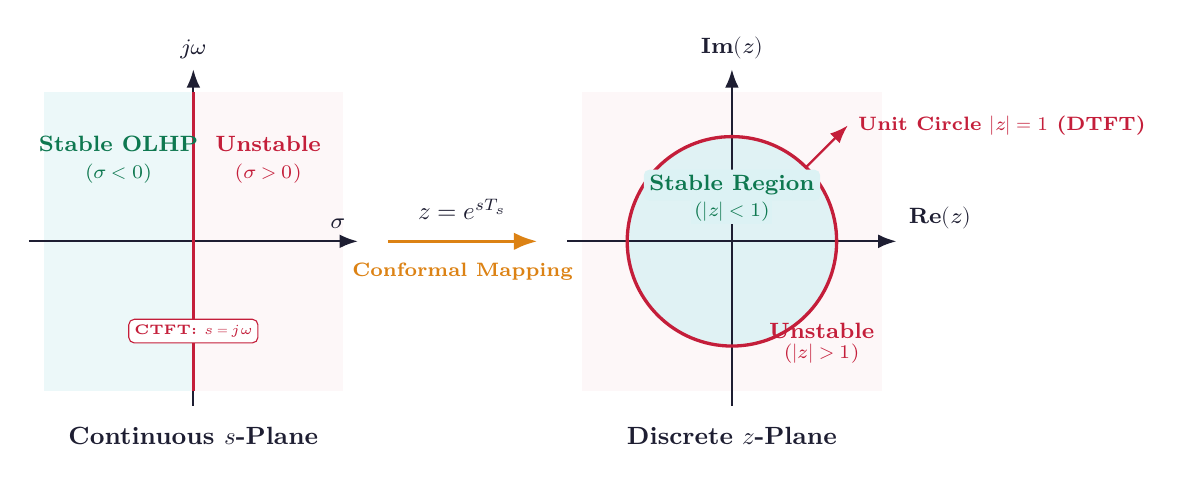
\begin{tikzpicture}[>=Latex, scale=0.95, font=\small]
  % ─── s-Plane (Continuous-Time) ───
  \begin{scope}[xshift=0cm]
    \fill[hdrteal, opacity=0.55] (-2.0,-2.0) rectangle (0,2.0);
    \fill[hdrred, opacity=0.35] (0,-2.0) rectangle (2.0,2.0);
    \draw[->, thick, color=mydark] (-2.2,0) -- (2.2,0) node[above left=1pt, font=\footnotesize\bfseries] {$\sigma$};
    \draw[->, thick, color=mydark] (0,-2.2) -- (0,2.3) node[above, font=\footnotesize\bfseries] {$j\omega$};
    \draw[very thick, myred] (0,-2.0) -- (0,2.0);
    \node[color=mygreen, font=\footnotesize\bfseries] at (-1.0,1.3) {Stable OLHP};
    \node[color=mygreen, font=\scriptsize] at (-1.0,0.9) {($\sigma < 0$)};
    \node[color=myred, font=\footnotesize\bfseries] at (1.0,1.3) {Unstable};
    \node[color=myred, font=\scriptsize] at (1.0,0.9) {($\sigma > 0$)};
    \node[draw=myred, fill=white, rounded corners=2pt, inner sep=2pt, font=\tiny\bfseries, text=myred] at (0,-1.2) {CTFT: $s = j\omega$};
    \node[below=4pt, font=\small\bfseries, color=mydark] at (0,-2.2) {Continuous $s$-Plane};
  \end{scope}

  % ─── Conformal Mapping Transition Arrow ───
  \draw[->, very thick, myamber, -{Latex[length=3mm]}] (2.6, 0) -- (4.6, 0)
    node[midway, above=4pt, font=\small\bfseries, color=mydark] {$z = e^{s T_s}$}
    node[midway, below=4pt, font=\scriptsize\bfseries, color=myamber] {Conformal Mapping};

  % ─── z-Plane (Discrete-Time) ───
  \begin{scope}[xshift=7.2cm]
    \fill[hdrred, opacity=0.35] (-2.0,-2.0) rectangle (2.0,2.0);
    \fill[hdrteal, opacity=0.85] (0,0) circle (1.4cm);
    \draw[->, thick, color=mydark] (-2.2,0) -- (2.2,0) node[above right=1pt, font=\footnotesize\bfseries] {$\text{Re}(z)$};
    \draw[->, thick, color=mydark] (0,-2.2) -- (0,2.3) node[above, font=\footnotesize\bfseries] {$\text{Im}(z)$};
    \draw[very thick, myred] (0,0) circle (1.4cm);
    \node[fill=hdrteal, rounded corners=2pt, inner sep=2pt, text=mygreen, font=\footnotesize\bfseries] at (0, 0.75) {Stable Region};
    \node[fill=hdrteal, inner sep=1pt, text=mygreen, font=\scriptsize] at (0, 0.40) {($|z| < 1$)};
    \node[color=myred, font=\footnotesize\bfseries] at (1.2, -1.2) {Unstable};
    \node[color=myred, font=\scriptsize] at (1.2, -1.5) {($|z| > 1$)};
    \draw[->, myred, thick] (0.99, 0.99) -- (1.55, 1.55) node[right, font=\scriptsize\bfseries, color=myred] {Unit Circle $|z|=1$ (DTFT)};
    \node[below=4pt, font=\small\bfseries, color=mydark] at (0,-2.2) {Discrete $z$-Plane};
  \end{scope}
\end{tikzpicture}
\end{center}
\end{tcolorbox}

% ───────────────────────────────────────────────────────────────────────────────
\section{The Laplace Transform}
% ───────────────────────────────────────────────────────────────────────────────

\subsection{Bilateral and Unilateral Laplace Transforms}

\begin{tcolorbox}[defbox, title={\textbf{Definition: Bilateral vs Unilateral Laplace Transform}}]
\begin{align}
  \textbf{Bilateral (Two-Sided):} \quad &X(s) = \mathcal{L}\{x(t)\} \triangleq \int_{-\infty}^{\infty} x(t) e^{-st} dt \\
  \textbf{Unilateral (Single-Sided):} \quad &X(s) = \mathcal{L}_u\{x(t)\} \triangleq \int_{0^-}^{\infty} x(t) e^{-st} dt
\end{align}
where $0^-$ includes impulses located at the origin $t=0$.
\end{tcolorbox}

\textbf{Why Unilateral Transform is Crucial for Engineers:}
\begin{itemize}[topsep=2pt, itemsep=2pt]
  \item Physical systems are causal, and experiments start at $t=0$.
  \item It naturally incorporates non-zero initial conditions ($y(0^-), y'(0^-)$), enabling algebraic solution of differential equations with initial stored energy.
\end{itemize}

\subsection{Eigenfunctions and Eigenfunction Basis}
As established in Module 3, $x(t) = e^{st}$ is an eigenfunction of an LSI system:
\begin{equation}
  y(t) = h(t) * e^{st} = \left[ \int_{-\infty}^{\infty} h(\tau) e^{-s\tau} d\tau \right] e^{st} = H(s) \cdot e^{st}
\end{equation}
The transfer function $H(s)$ is the eigenvalue. The continuum of eigenfunctions $\{e^{st}\}_{s \in \text{ROC}}$ forms a complete mathematical basis spanning the signal space of Laplace-transformable signals.

\subsection{Region of Convergence (ROC) for Laplace Transform}

\begin{tcolorbox}[defbox, title={\textbf{Definition: Region of Convergence (ROC)}}]
The \textbf{Region of Convergence (ROC)} is the set of complex values of $s = \sigma + j\omega$ in the $s$-plane for which the Laplace integral converges absolutely:
\begin{equation}
  \text{ROC} = \left\{ s \in \mathbb{C} : \int_{-\infty}^{\infty} |x(t)| e^{-\sigma t} dt < \infty \right\}
\end{equation}
\end{tcolorbox}

\textbf{Fundamental Properties of the Laplace ROC:}
\begin{enumerate}[topsep=2pt, itemsep=3pt]
  \item \textbf{Strip Geometry:} The ROC consists of vertical strips parallel to the $j\omega$-axis because convergence depends solely on $\sigma = \text{Re}(s)$, not on $\omega = \text{Im}(s)$.
  \item \textbf{Poles Exclusion:} The ROC contains \textbf{no poles} (since $X(s) \to \infty$ at poles).
  \item \textbf{Finite Duration Signals:} If $x(t)$ is non-zero only for $T_1 \le t \le T_2$ and is absolutely integrable, the ROC is the \textbf{entire $s$-plane}.
  \item \textbf{Right-Sided Signals:} If $x(t)$ is right-sided ($x(t) = 0$ for $t < T_1$), the ROC is a right-half plane:
  \begin{equation}
    \text{Re}(s) > \sigma_{\max} = \max_k\{\text{Re}(p_k)\}
  \end{equation}
  \item \textbf{Left-Sided Signals:} If $x(t)$ is left-sided ($x(t) = 0$ for $t > T_2$), the ROC is a left-half plane:
  \begin{equation}
    \text{Re}(s) < \sigma_{\min} = \min_k\{\text{Re}(p_k)\}
  \end{equation}
  \item \textbf{Two-Sided Signals:} If $x(t)$ is two-sided, the ROC is an open vertical strip: $\sigma_1 < \text{Re}(s) < \sigma_2$.
\end{enumerate}

\subsection{System Causality and Stability via ROC}

\begin{tcolorbox}[formulabox, title={\textbf{Causality and BIBO Stability Criteria in the \texorpdfstring{$s$}{s}-Plane}}]
\begin{enumerate}[topsep=2pt, itemsep=3pt]
  \item \textbf{Causality Criterion:} An LTI system is causal if and only if its ROC is a \textbf{right-half plane} extending to the right of the rightmost pole:
  \begin{equation}
    \text{ROC}: \quad \text{Re}(s) > \max_k\{\text{Re}(p_k)\}
  \end{equation}
  \item \textbf{BIBO Stability Criterion:} An LTI system is BIBO stable if and only if the \textbf{ROC includes the imaginary axis} ($j\omega$-axis, $\text{Re}(s) = 0$).
  \item \textbf{Causal + Stable Systems:} For an LTI system to be simultaneously causal and stable, \textbf{all poles must lie strictly in the Open Left-Half of the $s$-plane (OLHP)}:
  \begin{equation}
    \text{Re}(p_k) < 0 \quad \text{for all poles } p_k
  \end{equation}
\end{enumerate}
\end{tcolorbox}

\subsection{Poles, Zeros, and Transfer Function $H(s)$}
The transfer function of a rational continuous-time LSI system is:
\begin{equation}
  H(s) = \frac{Y(s)}{X(s)} = \frac{b_M s^M + b_{M-1} s^{M-1} + \dots + b_0}{a_N s^N + a_{N-1} s^{N-1} + \dots + a_0} = K \frac{\prod_{i=1}^M (s - z_i)}{\prod_{k=1}^N (s - p_k)}
\end{equation}
where:
\begin{itemize}[topsep=2pt, itemsep=2pt]
  \item $z_i$ are the \textbf{Zeros} (frequencies where $H(s) = 0$).
  \item $p_k$ are the \textbf{Poles} (frequencies where $H(s) \to \infty$).
  \item \textbf{Frequency Response Evaluation from Pole-Zero Vectors:}
  \begin{equation}
    |H(j\omega)| = |K| \frac{\prod_{i=1}^M |j\omega - z_i|}{\prod_{k=1}^N |j\omega - p_k|}, \qquad \angle H(j\omega) = \sum_{i=1}^M \angle(j\omega - z_i) - \sum_{k=1}^N \angle(j\omega - p_k)
  \end{equation}
\end{itemize}

\subsection{Solution of Differential Equations via Unilateral Laplace Transform}
The unilateral Laplace transform differentiation theorems state:
\begin{align}
  \mathcal{L}_u\left\{ \frac{dy(t)}{dt} \right\} &= s Y(s) - y(0^-) \\
  \mathcal{L}_u\left\{ \frac{d^2 y(t)}{dt^2} \right\} &= s^2 Y(s) - s y(0^-) - y'(0^-)
\end{align}
Applying this to an $N$-th order LCCDE yields:
\begin{equation}
  A(s) Y(s) - I(s) = B(s) X(s) \implies Y(s) = \underbrace{\frac{I(s)}{A(s)}}_{Y_{zi}(s) \text{ (ZIR)}} + \underbrace{\frac{B(s)}{A(s)} X(s)}_{Y_{zs}(s) \text{ (ZSR)}}
\end{equation}
where $I(s)$ contains all initial condition terms, and $H(s) = B(s)/A(s)$. Taking the inverse Laplace transform via Partial Fraction Expansion (PFE) yields the complete time-domain response $y(t) = y_{zi}(t) + y_{zs}(t)$.

% ───────────────────────────────────────────────────────────────────────────────
\section{The Z-Transform for Discrete-Time Signals and Systems}
% ───────────────────────────────────────────────────────────────────────────────

\subsection{Bilateral and Unilateral Z-Transforms}

\begin{tcolorbox}[defbox, title={\textbf{Definition: Bilateral vs Unilateral Z-Transform}}]
\begin{align}
  \textbf{Bilateral (Two-Sided):} \quad &X(z) = \mathcal{Z}\{x[n]\} \triangleq \sum_{n=-\infty}^{\infty} x[n] z^{-n} \\
  \textbf{Unilateral (Single-Sided):} \quad &X(z) = \mathcal{Z}_u\{x[n]\} \triangleq \sum_{n=0}^{\infty} x[n] z^{-n}
\end{align}
\end{tcolorbox}

\textbf{Eigenfunctions in Discrete-Time:}
The geometric sequence $x[n] = z^n$ ($z \in \mathbb{C}$) is the eigenfunction of DT LSI systems:
\begin{equation}
  y[n] = h[n] * z^n = \sum_{k=-\infty}^{\infty} h[k] z^{n-k} = z^n \left[ \sum_{k=-\infty}^{\infty} h[k] z^{-k} \right] = H(z) \cdot z^n
\end{equation}
The eigenvalue is the discrete system transfer function $H(z)$.

\subsection{Properties of the Region of Convergence (ROC) in the \texorpdfstring{$z$}{z}-Plane}

\begin{tcolorbox}[defbox, title={\textbf{Definition: ROC in the \texorpdfstring{$z$}{z}-Plane}}]
The ROC is the set of points in the complex $z$-plane for which the Laurent series converges absolutely:
\begin{equation}
  \text{ROC} = \left\{ z \in \mathbb{C} : \sum_{n=-\infty}^{\infty} |x[n]| \cdot |z|^{-n} < \infty \right\}
\end{equation}
\end{tcolorbox}

\textbf{Core Geometric Properties:}
\begin{enumerate}[topsep=2pt, itemsep=3pt]
  \item \textbf{Annular Rings:} The ROC is an open circular ring centered at the origin: $r_1 < |z| < r_2$.
  \item \textbf{No Poles in ROC:} The ROC cannot contain any poles.
  \item \textbf{Finite Length Sequences:} The ROC is the entire $z$-plane except possibly $z = 0$ (if $x[n]$ has non-zero values for $n > 0$) and/or $z = \infty$ (if $x[n]$ has non-zero values for $n < 0$).
  \item \textbf{Right-Sided Sequences:} If $x[n]$ is right-sided ($x[n] = 0$ for $n < N_1$), the ROC is the exterior of a circle:
  \begin{equation}
    |z| > r_{\max} = \max_k |p_k|
  \end{equation}
  \item \textbf{Left-Sided Sequences:} If $x[n]$ is left-sided ($x[n] = 0$ for $n > N_2$), the ROC is the interior of a circle:
  \begin{equation}
    |z| < r_{\min} = \min_k |p_k|
  \end{equation}
  \item \textbf{Two-Sided Sequences:} The ROC is an open annular ring between two concentric circles: $r_1 < |z| < r_2$.
\end{enumerate}

\subsection{Causality and Stability of DT LSI Systems}

\begin{tcolorbox}[formulabox, title={\textbf{Causality and BIBO Stability Criteria in the \texorpdfstring{$z$}{z}-Plane}}]
\begin{enumerate}[topsep=2pt, itemsep=3pt]
  \item \textbf{Causality Criterion:} A discrete-time LTI system is causal if and only if its ROC is the \textbf{exterior of a circle} outside the outermost pole, including $z = \infty$:
  \begin{equation}
    \text{ROC}: \quad |z| > \max_k |p_k|
  \end{equation}
  \item \textbf{BIBO Stability Criterion:} A discrete-time LTI system is BIBO stable if and only if the \textbf{ROC includes the unit circle} ($|z| = 1$).
  \item \textbf{Causal + Stable Systems:} For a DT system to be simultaneously causal and stable, \textbf{all poles must lie strictly inside the unit circle}:
  \begin{equation}
    |p_k| < 1 \quad \text{for all poles } p_k
  \end{equation}
\end{enumerate}
\end{tcolorbox}

\subsection{Common Z-Transform Pairs}

\par\vspace{6pt}\noindent
\begingroup
\setlength{\tabcolsep}{5pt}
\setlength{\extrarowheight}{3pt}
\renewcommand{\arraystretch}{1.4}
\begin{tabularx}{\linewidth}{|B{3.8cm}|B{4.5cm}|Y|}
\hline
\textbf{Sequence $x[n]$} & \textbf{Z-Transform $X(z)$} & \textbf{ROC} \\
\hline
$\delta[n]$ & $1$ & Entire $z$-plane \\
\hline
$u[n]$ & $\frac{1}{1 - z^{-1}} = \frac{z}{z - 1}$ & $|z| > 1$ \\
\hline
$-u[-n-1]$ & $\frac{1}{1 - z^{-1}} = \frac{z}{z - 1}$ & $|z| < 1$ \\
\hline
$a^n u[n]$ & $\frac{1}{1 - a z^{-1}} = \frac{z}{z - a}$ & $|z| > |a|$ \\
\hline
$-a^n u[-n-1]$ & $\frac{1}{1 - a z^{-1}} = \frac{z}{z - a}$ & $|z| < |a|$ \\
\hline
$n a^n u[n]$ & $\frac{a z^{-1}}{(1 - a z^{-1})^2} = \frac{a z}{(z - a)^2}$ & $|z| > |a|$ \\
\hline
$\cos(\Omega_0 n) u[n]$ & $\frac{1 - \cos(\Omega_0) z^{-1}}{1 - 2\cos(\Omega_0) z^{-1} + z^{-2}}$ & $|z| > 1$ \\
\hline
\end{tabularx}
\endgroup

\subsection{Z-Domain Analysis of Difference Equations}
The unilateral Z-transform time-delay properties incorporate initial conditions:
\begin{align}
  \mathcal{Z}_u\{y[n-1]\} &= z^{-1} Y(z) + y[-1] \\
  \mathcal{Z}_u\{y[n-2]\} &= z^{-2} Y(z) + z^{-1} y[-1] + y[-2]
\end{align}
Applying these to an $N$-th order difference equation $\sum_{k=0}^N a_k y[n-k] = \sum_{m=0}^M b_m x[n-m]$ transforms difference equations into algebraic equations in $z$, decomposing into Zero-Input Response (ZIR) and Zero-State Response (ZSR).

% ───────────────────────────────────────────────────────────────────────────────
% QUICK REVISION PAGE
% ───────────────────────────────────────────────────────────────────────────────
\newpage
\begin{center}
  {\Large\bfseries\color{myred} Quick Revision \& Examination Compendium}\\[3pt]
  {\small\color{watermark}\textbf{Module 4: Evolution of Transforms, Laplace \& Z-Transforms}}
\end{center}
\vspace{-2pt}
\noindent{\color{myred}\rule{\linewidth}{0.8pt}}

\begin{tcolorbox}[formulabox, title={\textbf{Key Formulas at a Glance}}]
\par\vspace{4pt}\noindent
\begingroup
\setlength{\tabcolsep}{5pt}
\setlength{\extrarowheight}{3pt}
\renewcommand{\arraystretch}{1.4}
\begin{tabularx}{\linewidth}{|B{4.5cm}|Y|}
\hline
\textbf{Transform / Property} & \textbf{Governing Mathematical Relation} \\
\hline
Bilateral Laplace Transform & $X(s) = \int_{-\infty}^{\infty} x(t) e^{-st} dt, \quad s = \sigma + j\omega$ \\
\hline
Unilateral Laplace Transform & $X(s) = \int_{0^-}^{\infty} x(t) e^{-st} dt$ \\
\hline
Laplace Derivative Property & $\mathcal{L}_u\{\dot{y}\} = s Y(s) - y(0^-), \quad \mathcal{L}_u\{\ddot{y}\} = s^2 Y - s y(0^-) - y'(0^-)$ \\
\hline
Continuous Causal+Stable Criterion & All poles in Open Left-Half Plane: $\text{Re}(p_k) < 0$ \\
\hline
Continuous Transfer Function & $H(s) = \mathcal{L}\{h(t)\} = Y(s) / X(s)$ \\
\hline
Bilateral Z-Transform & $X(z) = \sum_{n=-\infty}^{\infty} x[n] z^{-n}, \quad z = r e^{j\Omega}$ \\
\hline
Unilateral Z-Transform & $X(z) = \sum_{n=0}^{\infty} x[n] z^{-n}$ \\
\hline
Z-Transform Delay Property & $\mathcal{Z}_u\{y[n-1]\} = z^{-1} Y(z) + y[-1]$ \\
\hline
Discrete Causal+Stable Criterion & All poles inside Unit Circle: $|p_k| < 1$ \\
\hline
DTFT $\leftrightarrow$ Z-Transform & $X(e^{j\Omega}) = \left. X(z) \right|_{z = e^{j\Omega}} \quad (\text{if unit circle in ROC})$ \\
\hline
\end{tabularx}
\endgroup
\end{tcolorbox}

\begin{tcolorbox}[defbox, title={\textbf{One-Line Definitions for Rapid Review}}]
\par\vspace{4pt}\noindent
\begingroup
\setlength{\tabcolsep}{5pt}
\setlength{\extrarowheight}{3pt}
\renewcommand{\arraystretch}{1.35}
\begin{tabularx}{\linewidth}{|B{4.2cm}|Y|}
\hline
\textbf{Term} & \textbf{Definitive Technical Meaning} \\
\hline
Laplace Transform & A generalized Fourier transform with real damping factor $e^{-\sigma t}$ extending convergence to unstable signals. \\
\hline
Z-Transform & A generalized discrete-time Fourier transform with radial damping factor $r^{-n}$ extending convergence. \\
\hline
Region of Convergence (ROC) & The domain in the complex plane ($s$ or $z$) where the transform integral/series converges absolutely. \\
\hline
Poles of a System & Complex frequencies at which the transfer function denominator vanishes, causing infinite system gain. \\
\hline
Zeros of a System & Complex frequencies at which the transfer function numerator vanishes, completely blocking transmission. \\
\hline
Transfer Function $H(s) / H(z)$ & The ratio of the transform of the output to the transform of the input under zero initial conditions. \\
\hline
Open Left-Half Plane (OLHP) & The region $\text{Re}(s) < 0$ where all continuous-time system poles must lie for BIBO stability. \\
\hline
Unit Circle ($|z| = 1$) & The contour in the $z$-plane corresponding to the DTFT and the boundary of discrete-time BIBO stability. \\
\hline
Unilateral Transform & A transform defined strictly over non-negative time, tailored for causal systems and initial value problems. \\
\hline
\end{tabularx}
\endgroup
\end{tcolorbox}

\begin{tcolorbox}[exambox, title={\textbf{Frequently Asked / Viva Questions}}]
\begin{enumerate}[topsep=0pt, label=\textbf{Q\arabic*.}, itemsep=5pt]
  \item \Q{Why can the Fourier transform not handle the unit step function $u(t)$ directly without impulses?}
  Because $u(t)$ is not absolutely integrable ($\int_0^\infty 1 dt = \infty$). The convergence integral diverges on the imaginary axis. The Laplace transform introduces the factor $e^{-\sigma t}$ ($\sigma > 0$), forcing the integral to converge to $1/s$ in the ROC $\text{Re}(s) > 0$.

  \item \Q{Can two distinct time-domain signals have identical Laplace or Z-transform expressions?}
  Yes. For example, $x_1(t) = e^{-at}u(t)$ and $x_2(t) = -e^{-at}u(-t)$ both have the algebraic expression $1/(s+a)$. They are distinguished solely by their ROCs: $\text{Re}(s) > -a$ for $x_1(t)$ and $\text{Re}(s) < -a$ for $x_2(t)$. A transform is mathematically incomplete without specifying its ROC.

  \item \Q{State the condition on the ROC for an LTI system to be both causal and BIBO stable in continuous time.}
  The ROC must be a right-half plane $\text{Re}(s) > \sigma_{\max}$ (for causality), and it must contain the imaginary axis $\text{Re}(s) = 0$ (for stability). This implies that $\sigma_{\max} < 0$, meaning all poles must lie strictly in the Open Left-Half of the $s$-plane.

  \item \Q{What is the geometric mapping relationship between the $s$-plane and the $z$-plane?}
  The mapping is defined by $z = e^{s T_s}$. The imaginary axis $\text{Re}(s) = 0$ maps to the unit circle $|z| = 1$. The stable Open Left-Half Plane $\text{Re}(s) < 0$ maps to the interior of the unit circle $|z| < 1$. The unstable Right-Half Plane $\text{Re}(s) > 0$ maps to the exterior $|z| > 1$.

  \item \Q{What is the condition on poles for a causal discrete-time LTI system to be BIBO stable?}
  All poles must lie strictly inside the unit circle of the $z$-plane ($|p_k| < 1$ for all $k$).

  \item \Q{Why does the unilateral Laplace transform include initial conditions while the bilateral transform does not?}
  Because the integration begins at $t = 0^-$, the boundary values $y(0^-), y'(0^-)$ naturally emerge via integration by parts when evaluating derivatives, capturing internal stored energy.

  \item \Q{What is the physical interpretation of system zeros?}
  Zeros are frequencies where the system transmission is zero. If an input phasor has a frequency matching a zero ($s = z_i$), the steady-state output is completely extinguished.

  \item \Q{Why can a finite-duration signal have an ROC that is the entire complex plane?}
  For a signal of finite duration $[T_1, T_2]$, the integration/summation contains only finite limits. Provided the signal does not contain singularities of infinite area, the integral of $|x(t)|e^{-\sigma t}$ over a compact interval is always finite for any real $\sigma$.

  \item \Q{How do you determine the steady-state frequency response $H(j\omega)$ geometrically from the pole-zero plot?}
  At any point $j\omega$ on the imaginary axis, draw vectors from all zeros and poles to $j\omega$. The magnitude $|H(j\omega)|$ is the product of lengths of zero-vectors divided by the product of lengths of pole-vectors (scaled by gain $K$). The phase is the sum of angles of zero-vectors minus the sum of angles of pole-vectors.

  \item \Q{What is the Initial Value Theorem in the Laplace domain?}
  If $x(t)$ and its derivative are Laplace transformable and $x(t) = 0$ for $t < 0$, then $\lim_{t \to 0^+} x(t) = \lim_{s \to \infty} s X(s)$ (provided the limit exists).
\end{enumerate}
\end{tcolorbox}

\begin{tcolorbox}[tikzbox, title={\textbf{Summary Matrix: Comprehensive Comparison of Transforms}}]
\par\vspace{4pt}\noindent
\begingroup
\setlength{\tabcolsep}{4pt}
\setlength{\extrarowheight}{3pt}
\renewcommand{\arraystretch}{1.35}
\begin{tabularx}{\linewidth}{|B{2.5cm}|B{3.2cm}|B{3.2cm}|Y|}
\hline
\textbf{Transform} & \textbf{Kernel / Variable} & \textbf{Domain \& ROC} & \textbf{Stability Criterion} \\
\hline
CTFT & $e^{-j\omega t}, \quad \omega \in \mathbb{R}$ & Imaginary axis & Requires $\int |x(t)|dt < \infty$. \\
\hline
Laplace ($s$) & $e^{-st}, \quad s = \sigma + j\omega$ & Vertical strips in $s$-plane & ROC includes $j\omega$-axis (poles in OLHP). \\
\hline
DTFT & $e^{-j\Omega n}, \quad \Omega \in [-\pi, \pi]$ & Unit circle ($|z|=1$) & Requires $\sum |x[n]| < \infty$. \\
\hline
Z-Transform ($z$) & $z^{-n}, \quad z = r e^{j\Omega}$ & Annular rings in $z$-plane & ROC includes unit circle (poles inside $|z|<1$). \\
\hline
\end{tabularx}
\endgroup
\end{tcolorbox}


% -- Module 5 -----------------------------------------------------------------
\modulestart{5}{The Sampling Theorem}

\section{The Sampling Theorem}
% ───────────────────────────────────────────────────────────────────────────────

\subsection{Significance and Concept}
The sampling process forms the essential bridge connecting physical, continuous-time (analog) signals to discrete-time digital processors. The central question is: \textit{Under what conditions can a continuous signal be represented by discrete samples without any loss of information, and how can it be reconstructed exactly?}

\begin{tcolorbox}[defbox, title={\textbf{Nyquist-Shannon Sampling Theorem}}]
A continuous-time bandlimited signal $x(t)$ with finite energy and maximum frequency component $\omega_m$ (or $f_m = \omega_m / 2\pi$), such that:
\begin{equation}
  X(j\omega) = 0 \quad \text{for all } |\omega| > \omega_m
\end{equation}
can be uniquely, completely, and exactly reconstructed from its instantaneous samples $x(n T_s)$ taken at uniform time intervals $T_s$, if and only if the sampling frequency $\omega_s$ satisfies:
\begin{equation}
  \omega_s \ge 2 \omega_m \iff f_s \ge 2 f_m
\end{equation}
where $f_s = 1/T_s$ is the sampling rate in Hertz, and $\omega_s = 2\pi / T_s$ is in radians per second.
\end{tcolorbox}

\subsection{Key Sampling Terminology}
\begin{itemize}[topsep=2pt, itemsep=3pt]
  \item \textbf{Nyquist Rate ($f_N$):} The absolute minimum sampling rate required to avoid information loss:
  \begin{equation}
    f_N \triangleq 2 f_m \quad (\text{or } \omega_N \triangleq 2 \omega_m)
  \end{equation}
  \item \textbf{Nyquist Interval ($T_N$):} The maximum permissible time interval between consecutive samples:
  \begin{equation}
    T_N \triangleq \frac{1}{f_N} = \frac{1}{2 f_m} = \frac{\pi}{\omega_m}
  \end{equation}
  \item \textbf{Sampling Regimes:}
  \begin{enumerate}[topsep=2pt, itemsep=2pt]
    \item \textit{Over-sampling ($f_s > 2 f_m$):} Spectral replicas are separated by guard bands; exact reconstruction is easily achievable using practical filters.
    \item \textit{Critical sampling ($f_s = 2 f_m$):} Spectral replicas touch at edges without overlap; requires an ideal, infinitely sharp brick-wall filter.
    \item \textit{Under-sampling ($f_s < 2 f_m$):} Spectral replicas overlap, causing irreversible aliasing distortion.
  \end{enumerate}
\end{itemize}

% ───────────────────────────────────────────────────────────────────────────────
\section{Spectra of Sampled Signals (Impulse-Train Sampling)}
% ───────────────────────────────────────────────────────────────────────────────

\subsection{Mathematical Model of Ideal Sampling}
Ideal sampling is modeled as the product of the continuous-time analog signal $x(t)$ with a periodic Dirac impulse train $p(t)$:
\begin{equation}
  p(t) \triangleq \sum_{n=-\infty}^{\infty} \delta(t - n T_s)
\end{equation}
The sampled signal $x_p(t)$ is given by:
\begin{equation}
  x_p(t) = x(t) \cdot p(t) = x(t) \sum_{n=-\infty}^{\infty} \delta(t - n T_s) = \sum_{n=-\infty}^{\infty} x(n T_s) \delta(t - n T_s)
\end{equation}

\subsection{Spectral Derivation (Frequency Domain Analysis)}
To determine the Fourier transform of $x_p(t)$, we first express the periodic impulse train $p(t)$ in its Exponential Fourier Series:
\begin{equation}
  p(t) = \sum_{k=-\infty}^{\infty} c_k e^{j k \omega_s t}, \quad \text{where } c_k = \frac{1}{T_s} \int_{-T_s/2}^{T_s/2} \delta(t) e^{-j k \omega_s t} dt = \frac{1}{T_s}
\end{equation}
Thus, the Fourier transform of the sampling train is:
\begin{equation}
  P(j\omega) = \mathcal{F}\{p(t)\} = \frac{2\pi}{T_s} \sum_{k=-\infty}^{\infty} \delta(\omega - k \omega_s) = \omega_s \sum_{k=-\infty}^{\infty} \delta(\omega - k \omega_s)
\end{equation}
Applying the multiplication property of the CTFT ($\mathcal{F}\{x_1(t) x_2(t)\} = \frac{1}{2\pi} [X_1(j\omega) * X_2(j\omega)]$):
\begin{align}
  X_p(j\omega) &= \frac{1}{2\pi} \big[ X(j\omega) * P(j\omega) \big] \\
  &= \frac{1}{2\pi} \int_{-\infty}^{\infty} X(j\theta) \left[ \frac{2\pi}{T_s} \sum_{k=-\infty}^{\infty} \delta(\omega - \theta - k \omega_s) \right] d\theta
\end{align}
Interchanging integration and summation using the sifting property:

\begin{tcolorbox}[formulabox, title={\textbf{Core Formula: Spectrum of Sampled Signal}}]
\begin{equation}
  X_p(j\omega) = \frac{1}{T_s} \sum_{k=-\infty}^{\infty} X\big(j(\omega - k \omega_s)\big)
\end{equation}
\end{tcolorbox}

\textbf{Physical Meaning:}
Sampling in the time domain causes the original continuous spectrum $X(j\omega)$ to be \textbf{periodically replicated across the frequency axis} at integer multiples of the sampling frequency $\omega_s$, with each replica scaled by $1/T_s$.

\begin{tcolorbox}[tikzbox, title={\textbf{TikZ Illustration: Spectra of Continuous, Impulse Train, and Sampled Signals}}]
\begin{center}
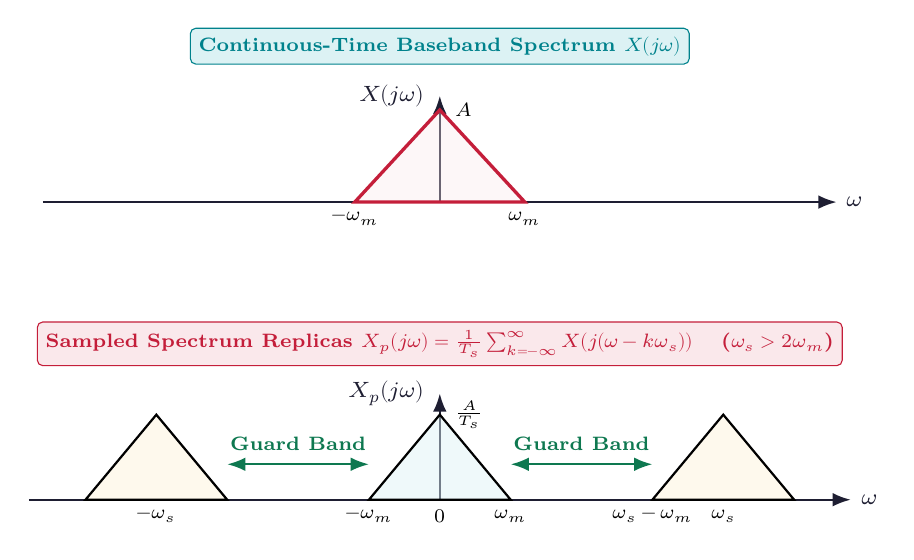
\begin{tikzpicture}[>=Latex, scale=0.90, font=\small]
  % ─── 1. Continuous Spectrum X(jw) ───
  \begin{scope}[yshift=4.2cm]
    \node[draw=myteal, fill=hdrteal, rounded corners=2pt, inner sep=3pt, font=\scriptsize\bfseries, text=myteal] at (0, 2.2) {Continuous-Time Baseband Spectrum $X(j\omega)$};
    \draw[->, thick, color=mydark] (-5.6,0) -- (5.6,0) node[right, font=\footnotesize] {$\omega$};
    \draw[->, thick, color=mydark] (0,0) -- (0,1.5) node[left=2pt, font=\footnotesize] {$X(j\omega)$};
    \draw[very thick, myred, fill=hdrred, fill opacity=0.35] (-1.2,0) -- (0,1.3) -- (1.2,0) -- cycle;
    \node[below, font=\scriptsize] at (-1.2,0) {$-\omega_m$};
    \node[below, font=\scriptsize] at (1.2,0) {$\omega_m$};
    \node[right=2pt, font=\scriptsize] at (0,1.3) {$A$};
  \end{scope}

  % ─── 2. Sampled Spectrum (Over-sampled: ws > 2 wm) ───
  \begin{scope}[yshift=0cm]
    \node[draw=myred, fill=hdrred, rounded corners=2pt, inner sep=3pt, font=\scriptsize\bfseries, text=myred] at (0, 2.2) {Sampled Spectrum Replicas $X_p(j\omega) = \frac{1}{T_s}\sum_{k=-\infty}^{\infty} X(j(\omega - k\omega_s))$ \quad ($\omega_s > 2\omega_m$)};
    \draw[->, thick, color=mydark] (-5.8,0) -- (5.8,0) node[right, font=\footnotesize] {$\omega$};
    \draw[->, thick, color=mydark] (0,0) -- (0,1.5) node[left=2pt, font=\footnotesize] {$X_p(j\omega)$};

    % Baseband k=0
    \draw[thick, fill=hdrteal, fill opacity=0.45] (-1.0,0) -- (0,1.2) -- (1.0,0) -- cycle;
    \node[below, font=\scriptsize] at (0,0) {$0$};
    \node[below, font=\scriptsize] at (-1.0,0) {$-\omega_m$};
    \node[below, font=\scriptsize] at (1.0,0) {$\omega_m$};
    \node[right=2pt, font=\scriptsize] at (0,1.2) {$\frac{A}{T_s}$};

    % Replica k=1 (center ws = 4.0)
    \draw[thick, fill=hdramber, fill opacity=0.45] (3.0,0) -- (4.0,1.2) -- (5.0,0) -- cycle;
    \node[below, font=\scriptsize] at (4.0,0) {$\omega_s$};
    \node[below, font=\scriptsize] at (3.0,0) {$\omega_s-\omega_m$};

    % Replica k=-1 (center -ws = -4.0)
    \draw[thick, fill=hdramber, fill opacity=0.45] (-5.0,0) -- (-4.0,1.2) -- (-3.0,0) -- cycle;
    \node[below, font=\scriptsize] at (-4.0,0) {$-\omega_s$};

    % Guard bands
    \draw[<->, mygreen, thick] (1.0,0.5) -- (3.0,0.5) node[midway, above=1pt, font=\scriptsize\bfseries, color=mygreen] {Guard Band};
    \draw[<->, mygreen, thick] (-3.0,0.5) -- (-1.0,0.5) node[midway, above=1pt, font=\scriptsize\bfseries, color=mygreen] {Guard Band};
  \end{scope}
\end{tikzpicture}
\end{center}
\end{tcolorbox}

% ───────────────────────────────────────────────────────────────────────────────
\section{Aliasing and Anti-Aliasing Techniques}
% ───────────────────────────────────────────────────────────────────────────────

\subsection{The Aliasing Phenomenon}
When a signal is sampled below the Nyquist rate ($\omega_s < 2\omega_m$), the adjacent spectral replicas overlap:
\begin{equation}
  \omega_s - \omega_m < \omega_m \implies \omega_s < 2\omega_m
\end{equation}
In the overlap regions, spectral components from high-frequency replicas fold into the baseband:

\begin{tcolorbox}[defbox, title={\textbf{Definition: Aliasing}}]
\textbf{Aliasing} is the spectral distortion phenomenon whereby high-frequency components of a continuous-time signal fold back across the Nyquist frequency ($f_s / 2$) and appear masquerading as indistinguishable lower-frequency components in the sampled signal.
\end{tcolorbox}

\begin{tcolorbox}[examplebox, title={\textbf{Demonstration: Aliased Frequency of a Sinusoid}}]
Consider a continuous sinusoidal tone $x(t) = \cos(2\pi f_0 t)$ sampled at rate $f_s$:
\begin{equation*}
  x[n] = x(n T_s) = \cos(2\pi f_0 n / f_s)
\end{equation*}
If $f_0 = 70\text{ Hz}$ and $f_s = 100\text{ Hz}$ (where Nyquist frequency is $f_s/2 = 50\text{ Hz}$):
\begin{align*}
  x[n] &= \cos\left(2\pi \frac{70}{100} n\right) = \cos(1.4\pi n) = \cos((2\pi - 0.6\pi) n) \\
  &= \cos(-0.6\pi n) = \cos(0.6\pi n) = \cos\left(2\pi \frac{30}{100} n\right)
\end{align*}
The 70~Hz signal appears identically as an apparent $30\text{ Hz}$ tone ($|f_0 - f_s| = |70 - 100| = 30\text{ Hz}$). The true high-frequency information is irrevocably corrupted.
\end{tcolorbox}

\subsection{Prevention of Aliasing: Anti-Aliasing Filter (AAF)}
Once aliasing occurs, the overlapping spectral components sum together linearly and \textbf{cannot be separated} by any post-processing algorithm. To prevent aliasing:
\begin{enumerate}[topsep=2pt, itemsep=2pt]
  \item \textbf{Pre-Filtering (Anti-Aliasing Filter):} An analog low-pass filter is inserted strictly \textit{before} the sampler. The filter has a cutoff frequency $f_c \le f_s / 2$, suppressing any input spectral energy exceeding the Nyquist foldover limit.
  \item \textbf{Over-sampling:} Selecting $f_s$ significantly higher than $2f_m$ widens the transition band for the analog anti-aliasing filter, allowing lower-order, cost-effective analog filter designs.
\end{enumerate}

% ───────────────────────────────────────────────────────────────────────────────
\section{Signal Reconstruction from Samples}
% ───────────────────────────────────────────────────────────────────────────────

\subsection{The Ideal Reconstruction Filter (Whittaker-Shannon Interpolation)}
When $\omega_s \ge 2\omega_m$, the original spectrum $X(j\omega)$ can be extracted from $X_p(j\omega)$ using an ideal low-pass filter with cutoff frequency $\omega_c$ ($\omega_m < \omega_c < \omega_s - \omega_m$) and gain $T_s$:
\begin{equation}
  H_r(j\omega) = \begin{cases} T_s, & |\omega| \le \frac{\omega_s}{2} \\ 0, & |\omega| > \frac{\omega_s}{2} \end{cases}
\end{equation}
The impulse response $h_r(t)$ of this ideal reconstruction filter is:
\begin{equation}
  h_r(t) = \mathcal{F}^{-1}\{H_r(j\omega)\} = \frac{T_s}{2\pi} \int_{-\omega_s/2}^{\omega_s/2} e^{j\omega t} d\omega = \frac{T_s}{2\pi} \left[ \frac{e^{j\omega t}}{jt} \right]_{-\pi/T_s}^{\pi/T_s} = \frac{\sin(\pi t / T_s)}{\pi t / T_s} = \text{sinc}\left(\frac{t}{T_s}\right)
\end{equation}
Convolving the sampled impulse train $x_p(t)$ with $h_r(t)$ yields:

\begin{tcolorbox}[formulabox, title={\textbf{Whittaker-Shannon Cardinal Reconstruction Formula}}]
\begin{equation}
  x(t) = x_p(t) * h_r(t) = \sum_{n=-\infty}^{\infty} x(n T_s) \text{sinc}\left(\frac{t - n T_s}{T_s}\right)
\end{equation}
where $\text{sinc}(u) \triangleq \frac{\sin(\pi u)}{\pi u}$.
\end{tcolorbox}

\textbf{Geometric Interpolation Property:}
At the exact sampling instants $t = m T_s$:
\begin{equation}
  \text{sinc}\left(\frac{m T_s - n T_s}{T_s}\right) = \text{sinc}(m - n) = \begin{cases} 1, & m = n \\ 0, & m \ne n \end{cases}
\end{equation}
Thus, at each sampling point, the reconstructed signal equals the exact sample value $x(m T_s)$ because all neighboring sinc interpolation curves pass through zero.

\textbf{Practical Limitation:} The ideal sinc interpolator is \textbf{physically unrealizable} because $\text{sinc}(t/T_s)$ has infinite duration, requiring knowledge of all past and future samples ($h_r(t) \ne 0$ for $t < 0$, non-causal).

\subsection{Zero-Order Hold (ZOH)}
In practical digital-to-analog converters (DACs), the simplest and most ubiquitous hold device is the \textbf{Zero-Order Hold (ZOH)}, which clamps each sample value until the arrival of the next sample:
\begin{equation}
  x_{zoh}(t) = x(n T_s) \quad \text{for } n T_s \le t < (n+1)T_s
\end{equation}

\begin{itemize}[topsep=2pt, itemsep=2pt]
  \item \textbf{Impulse Response:} A causal rectangular pulse of duration $T_s$:
  \begin{equation}
    h_0(t) = u(t) - u(t - T_s) = \text{rect}\left(\frac{t - T_s/2}{T_s}\right)
  \end{equation}
  \item \textbf{Frequency Response:}
  \begin{equation}
    H_0(j\omega) = \int_0^{T_s} e^{-j\omega t} dt = \frac{1 - e^{-j\omega T_s}}{j\omega} = T_s \left( \frac{\sin(\omega T_s / 2)}{\omega T_s / 2} \right) e^{-j\omega T_s / 2} = T_s \text{sinc}\left(\frac{\omega T_s}{2\pi}\right) e^{-j\omega T_s / 2}
  \end{equation}
  \item \textbf{Distortion Effects of ZOH:}
  \begin{enumerate}[topsep=2pt, itemsep=2pt]
    \item \textit{In-band Droop (Sinc Roll-off):} Magnitude response attenuates at the band edge $\omega_s/2$ by a factor of $\text{sinc}(0.5) = \frac{2}{\pi} \approx 0.637$ ($-3.92\text{ dB}$).
    \item \textit{High-Frequency Images:} The sinc side-lobes decay slowly ($\propto 1/\omega$), leaving residual harmonic images. A post-reconstruction smoothing filter and equalization circuit ($\frac{1}{\text{sinc}}$) are required.
  \end{enumerate}
\end{itemize}

\subsection{First-Order Hold (FOH)}
The \textbf{First-Order Hold (FOH)} performs linear extrapolation/interpolation between consecutive sample points.
\begin{itemize}[topsep=2pt, itemsep=2pt]
  \item \textbf{Impulse Response (Triangular Pulse):}
  \begin{equation}
    h_1(t) = \begin{cases} 1 - \frac{|t|}{T_s}, & |t| \le T_s \\ 0, & |t| > T_s \end{cases}
  \end{equation}
  \item \textbf{Frequency Response:}
  \begin{equation}
    H_1(j\omega) = T_s \left( \frac{\sin(\omega T_s / 2)}{\omega T_s / 2} \right)^2 = T_s \text{sinc}^2\left(\frac{\omega T_s}{2\pi}\right)
  \end{equation}
  \item \textbf{Advantage:} The side-lobes decay as $1/\omega^2$, providing vastly superior suppression of spectral images compared to ZOH. (A causal implementation requires 1 sample delay $T_s$).
\end{itemize}

% ───────────────────────────────────────────────────────────────────────────────
\section{Relation Between Continuous and Discrete-Time Systems}
% ───────────────────────────────────────────────────────────────────────────────

\subsection{Mapping of Time and Frequency Variables}
When a continuous signal $x_c(t)$ is sampled with period $T_s$, the discrete-time sequence is $x[n] = x_c(n T_s)$. The independent variables are related by:
\begin{equation}
  t = n T_s = \frac{n}{f_s}
\end{equation}
The relationship between continuous-time angular frequency $\omega$ (rad/s) and discrete-time angular frequency $\Omega$ (rad/sample) is:
\begin{equation}
  \Omega = \omega T_s = \frac{\omega}{f_s} = 2\pi \frac{f}{f_s}
\end{equation}

\textbf{Key Frequency Correspondence:}
\begin{itemize}[topsep=2pt, itemsep=2pt]
  \item Continuous DC ($\omega = 0$) maps to Discrete DC ($\Omega = 0$).
  \item Continuous Nyquist frequency ($\omega = \omega_s / 2 = \pi / T_s$) maps directly to the discrete half-sample frequency $\Omega = \pi$.
  \item Sampling frequency $\omega = \omega_s$ maps to $\Omega = 2\pi$ (which is identical to $0$ due to $2\pi$-periodicity).
\end{itemize}

\subsection{Digital Processing of Continuous-Time Signals}
A standard digital signal processing (DSP) system architecture comprises:
\begin{equation*}
  x_c(t) \xrightarrow{\text{AAF}} x_a(t) \xrightarrow{\text{C/D}} x[n] \xrightarrow{\boxed{H(e^{j\Omega})}} y[n] \xrightarrow{\text{D/C}} y_c(t)
\end{equation*}
If sampling satisfies the Nyquist condition ($f_s \ge 2 f_m$), the overall continuous-time system behaves as an equivalent LTI analog filter with effective frequency response:
\begin{equation}
  H_{eff}(j\omega) = \begin{cases} \left. H(e^{j\Omega}) \right|_{\Omega = \omega T_s}, & |\omega| < \frac{\pi}{T_s} \\ 0, & |\omega| \ge \frac{\pi}{T_s} \end{cases}
\end{equation}

% ───────────────────────────────────────────────────────────────────────────────
% QUICK REVISION PAGE
% ───────────────────────────────────────────────────────────────────────────────
\newpage
\begin{center}
  {\Large\bfseries\color{myred} Quick Revision \& Examination Compendium}\\[3pt]
  {\small\color{watermark}\textbf{Module 5: The Sampling Theorem \& Signal Reconstruction}}
\end{center}
\vspace{-2pt}
\noindent{\color{myred}\rule{\linewidth}{0.8pt}}

\begin{tcolorbox}[formulabox, title={\textbf{Key Formulas at a Glance}}]
\par\vspace{4pt}\noindent
\begingroup
\setlength{\tabcolsep}{5pt}
\setlength{\extrarowheight}{3pt}
\renewcommand{\arraystretch}{1.4}
\begin{tabularx}{\linewidth}{|B{4.5cm}|Y|}
\hline
\textbf{Concept / Law} & \textbf{Definitive Mathematical Formula} \\
\hline
Nyquist Sampling Criterion & $f_s \ge 2 f_m \iff \omega_s \ge 2 \omega_m$ \\
\hline
Nyquist Rate & $f_N = 2 f_m \quad (\text{Hz}), \quad \omega_N = 2 \omega_m \quad (\text{rad/s})$ \\
\hline
Nyquist Interval & $T_N = \frac{1}{2 f_m} = \frac{\pi}{\omega_m} \quad (\text{seconds})$ \\
\hline
Sampled Spectrum Replication & $X_p(j\omega) = \frac{1}{T_s} \sum_{k=-\infty}^{\infty} X\big(j(\omega - k \omega_s)\big)$ \\
\hline
Aliased Frequency & $f_{apparent} = |f_0 - k f_s| \le \frac{f_s}{2}$ \\
\hline
Ideal Sinc Interpolation & $x(t) = \sum_{n=-\infty}^{\infty} x(n T_s) \text{sinc}\left(\frac{t - n T_s}{T_s}\right)$ \\
\hline
Zero-Order Hold Transfer Function & $H_0(j\omega) = T_s \left(\frac{\sin(\omega T_s / 2)}{\omega T_s / 2}\right) e^{-j\omega T_s / 2}$ \\
\hline
First-Order Hold Transfer Function & $H_1(j\omega) = T_s \text{sinc}^2\left(\frac{\omega T_s}{2\pi}\right)$ \\
\hline
CT to DT Frequency Mapping & $\Omega = \omega T_s = \frac{\omega}{f_s}$ \\
\hline
Effective DSP Frequency Response & $H_{eff}(j\omega) = H(e^{j\omega T_s}) \quad \text{for } |\omega| < \frac{\pi}{T_s}$ \\
\hline
\end{tabularx}
\endgroup
\end{tcolorbox}

\begin{tcolorbox}[defbox, title={\textbf{One-Line Definitions for Rapid Review}}]
\par\vspace{4pt}\noindent
\begingroup
\setlength{\tabcolsep}{5pt}
\setlength{\extrarowheight}{3pt}
\renewcommand{\arraystretch}{1.35}
\begin{tabularx}{\linewidth}{|B{4.2cm}|Y|}
\hline
\textbf{Term} & \textbf{Definitive Technical Meaning} \\
\hline
Sampling Theorem & Principle stating a bandlimited signal can be perfectly recovered if sampled at $\ge 2\times$ maximum frequency. \\
\hline
Nyquist Rate & The minimum theoretical sampling frequency ($2f_m$) required to avoid spectral overlap and aliasing. \\
\hline
Aliasing & An irreversible distortion where high frequencies fold into lower bands due to inadequate sampling rates. \\
\hline
Anti-Aliasing Filter & An analog low-pass pre-filter that removes signal content above $f_s/2$ prior to sampling. \\
\hline
Whittaker-Shannon Interpolation & The mathematically exact reconstruction formula using weighted, time-shifted sinc functions. \\
\hline
Zero-Order Hold (ZOH) & A DAC reconstruction filter that holds each sample amplitude flat over the entire sampling interval. \\
\hline
First-Order Hold (FOH) & A reconstruction filter that performs linear triangular interpolation between consecutive sample points. \\
\hline
Guard Band & The frequency separation gap $(\omega_s - 2\omega_m)$ between adjacent spectral replicas in over-sampled systems. \\
\hline
Anti-Imaging Filter & A post-DAC analog smoothing filter designed to suppress high-frequency periodic images from the hold circuit. \\
\hline
\end{tabularx}
\endgroup
\end{tcolorbox}

\begin{tcolorbox}[exambox, title={\textbf{Frequently Asked / Viva Questions}}]
\begin{enumerate}[topsep=0pt, label=\textbf{Q\arabic*.}, itemsep=5pt]
  \item \Q{What is the Nyquist rate for the composite signal $x(t) = 3\cos(100\pi t) + 2\sin(300\pi t) - 5\cos(200\pi t)$?}
  Identify the angular frequencies: $\omega_1 = 100\pi \implies f_1 = 50\text{ Hz}$, $\omega_2 = 300\pi \implies f_2 = 150\text{ Hz}$, $\omega_3 = 200\pi \implies f_3 = 100\text{ Hz}$. The highest frequency is $f_m = 150\text{ Hz}$. Thus, Nyquist rate $f_N = 2 f_m = 2 \times 150 = 300\text{ Hz}$ (or $\omega_N = 600\pi\text{ rad/s}$).

  \item \Q{What is the Nyquist rate for $x(t) = \text{sinc}(100 t) \cdot \text{sinc}(200 t)$?}
  In the frequency domain, multiplication in time corresponds to convolution: $X(j\omega) = \frac{1}{2\pi} [X_1(j\omega) * X_2(j\omega)]$. The bandwidths of the rectangular spectra add: $W = W_1 + W_2 = 100\pi + 200\pi = 300\pi\text{ rad/s}$. Thus, $f_m = 150\text{ Hz}$, giving Nyquist rate $f_N = 2 f_m = 300\text{ Hz}$.

  \item \Q{Why cannot an aliased signal be corrected or de-aliased digitally after sampling?}
  Once aliasing occurs, overlapping high- and low-frequency spectral components sum together into identical frequency bins in the sampled sequence. Since a single composite sum contains no tag indicating individual source components, separation is mathematically impossible.

  \item \Q{Why is an Anti-Aliasing Filter placed before the sampler rather than after?}
  Because aliasing occurs during the sampling operation itself. Placing the filter after the sampler attempts to filter a signal that is already contaminated with folded noise that now resides in the legitimate signal band.

  \item \Q{Why is ideal sinc interpolation practically unrealizable?}
  Because $\text{sinc}(t/T_s) = \frac{\sin(\pi t / T_s)}{\pi t / T_s}$ has infinite duration extending from $t = -\infty$ to $+\infty$. Realizing it would require infinite delay and infinite non-causal memory.

  \item \Q{What is the passband droop caused by a Zero-Order Hold (ZOH)?}
  The ZOH frequency response has magnitude $|H_0(j\omega)| = T_s \left|\frac{\sin(\omega T_s / 2)}{\omega T_s / 2}\right|$. At the band edge $\omega = \omega_s / 2$, $|H_0| = T_s \frac{\sin(\pi/2)}{\pi/2} = \frac{2}{\pi} T_s \approx 0.637 T_s$. This produces an in-band attenuation of $20\log_{10}(2/\pi) \approx -3.92\text{ dB}$, requiring an inverse-sinc equalizer.

  \item \Q{Compare ZOH and FOH in terms of spectral image suppression.}
  ZOH has side-lobes that decay at a rate of $1/\omega$ ($-20\text{ dB/decade}$), whereas FOH has side-lobes that decay at $1/\omega^2$ ($-40\text{ dB/decade}$). FOH provides vastly superior attenuation of high-frequency images.

  \item \Q{What continuous frequency $\omega$ corresponds to $\Omega = \pi$ in a discrete-time system?}
  $\Omega = \omega T_s = \pi \implies \omega = \frac{\pi}{T_s} = \frac{\omega_s}{2} = \pi f_s$. This corresponds precisely to the continuous-time Nyquist foldover frequency.

  \item \Q{What is meant by flat-top sampling and how does it differ from natural sampling?}
  In natural sampling, the tops of the sampled pulses follow the exact analog contour of $x(t)$. In flat-top sampling, each pulse has a constant (flat) amplitude equal to the sample value at the pulse onset. Flat-top sampling introduces aperture distortion ($\text{sinc}$ attenuation) similar to a sample-and-hold circuit.

  \item \Q{What is the Nyquist rate for $x(t) = \cos^2(400\pi t)$?}
  Using the trigonometric identity: $\cos^2(\theta) = \frac{1 + \cos(2\theta)}{2}$. Thus, $x(t) = \frac{1}{2} + \frac{1}{2}\cos(800\pi t)$. The maximum frequency is $f_m = 400\text{ Hz}$. Hence, the Nyquist rate is $f_N = 2 f_m = 800\text{ Hz}$.
\end{enumerate}
\end{tcolorbox}

\begin{tcolorbox}[tikzbox, title={\textbf{Summary Matrix: Comparison of Signal Reconstruction Methods}}]
\par\vspace{4pt}\noindent
\begingroup
\setlength{\tabcolsep}{4.5pt}
\setlength{\extrarowheight}{3pt}
\renewcommand{\arraystretch}{1.35}
\begin{tabularx}{\linewidth}{|B{3.2cm}|B{3.8cm}|B{3.2cm}|Y|}
\hline
\textbf{Reconstruction Filter} & \textbf{Impulse Response $h(t)$} & \textbf{Frequency Response} & \textbf{Practical Feasibility} \\
\hline
Ideal Sinc Interpolator & $\text{sinc}(t / T_s)$ & Ideal brick-wall boxcar & Unrealizable; non-causal, infinite delay. \\
\hline
Zero-Order Hold (ZOH) & $\text{rect}\left(\frac{t - T_s/2}{T_s}\right)$ (Staircase) & $T_s \text{sinc}\left(\frac{\omega T_s}{2\pi}\right) e^{-j\omega T_s/2}$ & Universal in DACs; causes $-3.92\text{ dB}$ droop. \\
\hline
First-Order Hold (FOH) & $\text{tri}\left(\frac{t}{T_s}\right)$ (Linear interpolation) & $T_s \text{sinc}^2\left(\frac{\omega T_s}{2\pi}\right)$ & Causal with 1 sample delay; $-40\text{ dB/dec}$ rolloff. \\
\hline
\end{tabularx}
\endgroup
\end{tcolorbox}


\end{document}
